\documentclass{article}
\usepackage{cmap}
\usepackage{mathtext}
\usepackage[T2A]{fontenc}
\usepackage[utf8]{inputenc}        
\usepackage[english,russian]{babel}
\usepackage{epigraph}
\usepackage{fancybox,fancyhdr}
\usepackage{multicol}
\usepackage{float}
\usepackage{venndiagram}
\usepackage{mathtools}
\usepackage{nicefrac}
\usepackage[top=0.7in, bottom=0.75in, left=0.625in, right=0.625in]{geometry}
\usepackage{ytableau}
\usepackage{amsmath,amssymb}
\DeclareMathOperator{\Exists}{\exists}
\DeclareMathOperator{\eps}{\varepsilon}
\DeclareMathOperator{\Forall}{\forall}
\DeclareMathOperator{\re}{\mathbb{R}}
\DeclareMathOperator{\z}{\mathbb{Z}}
\DeclareMathOperator{\n}{\mathbb{N}}
\usepackage{tikz}
\usetikzlibrary{positioning,chains,fit,shapes,calc}
\newcommand\abs[1]{\left|#1\right|}
 
\title{Вопросы к коллоквиуму-1 по матанализу}
\author{}
\date{1 декабря 2018}
 
\begin{document}
\normalsize
\maketitle
\setcounter{section}{20}
 
\begin{center}
    По вопросам к теху обращайтесь:
    \begin{enumerate}
        \item Вопросы 1-10: Бабушанова Даша
        \item Вопросы 11-20: Юрлов Павел
        \item Вопросы 21-30: Стрельцов Артем
        \item Вопросы 31-38: Дегтеринский Николай
    \end{enumerate}
\end{center}
 
 
%tic1
\section*{Вопрос 1}
   
\begin{center}
    Аксиомы множества вещественных чисел. Аксиомы непрерывности.
\end{center}
 
   \textbf{Определение: }Вещественные числа - множество элементов ($\mathbb{R}$) на котором задано 2 базовых операции (<<+>> и <<$\times$>>) и отношение порядка <<$\leqslant$>>, которые удовлетворяют набору аксиом.
\begin{center}
   
\end{center}
 
\begin{center}
   \textbf{Аксиомы сложения:}
\end{center}
 
\begin{center}
       1) $\forall a,b \in \mathbb{R}$: a + b = b + a \\
       2) $\forall a,b,c \in \mathbb{R}$: (a + b) + c = a + (b + c) \\
       3) $\Exists 0 \in \mathbb{R} $ $ \forall a \in \mathbb{R}$: a + 0 = 0 + a = a \\
       4) $\forall a \in \mathbb{R} $ $ \Exists (-a) \in \mathbb{R}$: a + (-a) = (-a) + a = 0\\
\end{center}
 
\begin{center}
   \textbf{Аксиомы умножения:}
\end{center}
 
\begin{center}
   5) $\forall a,b \in \mathbb{R}$: ab = ba \\
   6) $\forall a,b,c \in \mathbb{R}$: a(bc) = (ab)c \\
   7) $\exists 1 \in \mathbb{R}$: $a\cdot 1 = 1 \cdot a = a$ \\
   8) $\forall a \in \mathbb{R}$, $a \neq 0$: $\Exists 1/a \in \mathbb{R}$: $a \cdot (1/a) = 1$\\
   (1/a - обратное для а) \\
\end{center}
\newpage
\begin{center}
   \textbf{Аксиома связи <<+>> и <<$\times$>>:}
\end{center}
\begin{center}
   9) $\forall a,b,c \in \mathbb{R}$: $a\cdot(b + c)$ = ab + ac\\
\end{center}
 
\begin{center}
   \textbf{Аксиомы сравнения:}
\end{center}
 
\begin{center}
   10) $\forall a,b \in \mathbb{R}$: $ a \leq b $ и $ b \leq a \Rightarrow  a = b $ \\
   11) $\forall a,b \in \mathbb{R}$: $ a \leq b$ и $ b \leq c \Rightarrow a \leq c $ \\
\end{center}
 
\begin{center}
   \textbf{Связь порядка и сложения:}
\end{center}
 
\begin{center}
   12) $\forall a,b,c \in \mathbb{R}$: $ a \leq b \Rightarrow (a + c) \leq (b + c)$ \\
\end{center}
 
\begin{center}
   \textbf{Cвязь порядка и умножения:}
\end{center}
 
\begin{center}
   13) $\forall a,b \in \mathbb{R}$: $ 0 \leq a $ и $ 0 \leq b \Rightarrow 0 \leq ab $ \\
\end{center}
 
\begin{center}
   \textbf{Аксиома непрерывности:}
\end{center}
 
\begin{center}
   14) Для $\forall $ непустых подможеств $A,B \subset \mathbb{R} $ с условием $ \Forall a \in A$ и $\forall b \in B$, $ a \leq b $ \\
   $\Exists c \in \mathbb{R}$ $\Forall a \in A $ и $ b \in B$: \\
   $ a \leq c \leq b $
\end{center}
\bigskip\bigskip
%tic2
\section*{Вопрос 2}
 
\begin{center}
   {Определение точной верхней и точной нижней граней ограниченного числового множества. Существование точной верхней грани (как следствие из аксиомы непрерывности). Единственность точней верхней грани.}
\end{center}
   1. A - множество ограниченное сверху. \\
   Число $d \in R $ называется точной верхней гранью (супремумом) множества $А$, если: \\
   1) d - верхняя грань \\
   2) $\Forall  c < d $  не является верхней гранью для $А$ \\
   Иначе говоря, $d = \sup A$, если:\\
   1) $\Forall a \in A$, $ a \leq d $ \\
   2) $\Forall c < d$ $\Exists a \in A$, $a > c $\\
   \\
   2. \textbf{У ограниченного сверху мн-ва существует супремум.}\\
   Рассмотрим $В$ =  \{мн-во всех верхних граней мн-ва А\}
   =  $\{b \in \mathbb{R} | \forall a \in A, a \leq b  \}$, $A,B \neq \emptyset$ \\
   По аксиоме (14): $\Exists d \in \mathbb{R}$ :  $ a \leq d \leq b  \Rightarrow d$ - $\sup A$ \\
   Возьмем $ c < d$:  Допустим, что $с$ - верхняя грань, тогда $ с \in B$, \\
   но $\forall b \in B$ $b \geqslant d \Rightarrow c \geqslant d $. \\
   Противоречие. \\
   \\
   3. \textbf{Супремум  единственный}\\
    Пусть множество A  имеет 2 точных верхних грани: $ a_1 $ и $ a_2$.\\
    Допустим, что $ a_1 < a_2$. Так как $a_1 < a_2$ и $a_2$ = supA, то $\Exists a' \in A$: a' > $ a_1$, что противоречит тому факту, что $ a_1  = \sup A$.
 
\bigskip\bigskip
%tic3
\section*{Вопрос 3}
 
\begin{center}
  {Бесконечные десятичные дроби (бдд). Сравнение бдд. Алгоритм построения точной верхней грани для множества положительных бдд, ограниченного сверху.}
\end{center}
 
   Бдд - выражение вида $\alpha$ = $\pm \alpha_0$,$\alpha_1\alpha_2$..., где $\alpha_0 \in $ \{0,1,2..\};
   $\alpha_n \in$ \{0,1,2.. 9\}\\
   \\
   \textbf{Сравнение бдд:}\\
   1. Пусть $\alpha \geq 0$, $ \beta \geq 0$: \\
       $\alpha$ = $\alpha_0$, $\alpha_1$ $\alpha_2$... \\
       $\beta$ = $\beta_0$, $\beta_1$ $\beta_2$... \\
       Скажем, что $\alpha$ < $\beta$, если выполнено хотя бы одно утверждение: \\
       $\cdot  \alpha_0$ < $\beta_0$ \\
       $\cdot  \alpha_0$ = $\beta_0$, $\alpha_1$ < $\beta_1$ \\
       $\cdot  \alpha_0$ = $\beta_0$, $\alpha_1$ = $\beta_1$, $\alpha_2$ < $\beta_2$ \\
       $\cdot$ \\
       $\cdot$ \\
       Иначе $ \alpha$ > $\beta$. \\
   2. Если $\alpha$ < 0  и $\beta$ > 0: $\alpha$ < $\beta$. \\
   3. Если $\alpha \leq 0 $ и $ \beta \leq 0$, - $\alpha$ < - $\beta$ (преобразуем в положительные бдд, а потом используем первый пункт) $ \rightarrow  \alpha$ > $\beta$. \\
   \\
   \textbf{Определим точную верхнюю грань множества бдд:} \\
   Пусть X - ограниченное множество бдд.
   (т.е. $\Exists$ с такая, что $\Forall x \in X$: $ x \leq c$.) \\
   Определим $\beta$ = $\beta_0$, $\beta_1$ $\beta_2$... = supX. \\
   \\
   \textbf{Приведем алгоритм: } \\
   $\beta_0$ = max\{ $\alpha_0$ | $\alpha \in X$ \} \\
   $A_1$ = \{ $\alpha \in X$ | $ \alpha_0 = \beta_0$ \} \\
   $\beta_1$ = max\{$\alpha_1$ | $\alpha \in A_1$ \} \\
   $A_2$ = \{ $\alpha \in A_1$ | $ \alpha_1 = \beta_1$ \} \\
   $\beta_2$ = max\{$\alpha_2$ | $\alpha \in A_2$ \} \\
   $A_3$ = \{ $\alpha \in A_2$ | $ \alpha_2 = \beta_2$ \} \\
 
%tic4
\section*{Вопрос 4}
 
\begin{center}
 {Построение арифметических опрераций на множестве бдд на примере суммы двух положительных бдд.}
\end{center}
 
   $\alpha$ = $\alpha_0$, $\alpha_1$ $\alpha_2$... > 0\\
   $\beta$ = $\beta_0$, $\beta_1$ $\beta_2$... > 0\\
   \\
   \textbf{Определим сумму бдд: }\\
   $\alpha$ + $\beta$ = sup \{ x + y | $ 0 \leq x \leq \alpha $, x - конечная десятичная дробь, \\
   $ 0 \leq y \leq \beta $, y - конечная десятичная дробь\} \\
   \\
   \textbf{Определим умножение бдд} (на всяких случай)\textbf{:} \\
   $\alpha \cdot \beta$ = sup \{ $x \cdot y $ | $ 0 \leq x \leq \alpha $, x - конечная десятичная дробь, \\
   $ 0 \leq y \leq \beta $, y - конечная десятичная дробь\} \\
\newpage
%tic5
\section*{Вопрос 5}
 
\begin{center}
   {Теорема о единственности множества вещественных чисел с точностью до изоморфизма (без доказательства).}
\end{center}
 
   \textbf{Теорема о единственности множества вещественных чисел.} \\
   Пусть $\mathbb{R}$ и $ (\widetilde{\mathbb{R}})$ - множества, удовлетворяющие всем аксиомам 1 - 14. Тогда имеется биекция $\mathbb{R} \rightarrow (\widetilde{\mathbb{R}})$, такая что: \\
   p : $\mathbb{R} \rightarrow \widetilde{\mathbb{R}}$ \\
   $\cdot $ x + y $\Longleftrightarrow \tilde{x} + \tilde{y} $ | p(x + y) = p(x) + p(y); \\
   $\cdot $ xy $\Longleftrightarrow \tilde{x} \tilde{y}$ |  p(xy) = p(x) $\cdot$ p(y); \\
   $\cdot$  $x \leq y \Longleftrightarrow \tilde{x} \leq \tilde{y} $ | если $x \leq y$: $p(x) \leq p(y)$, $\Forall x,y \in \mathbb{R}$; \\
 
%tic6
\section*{Вопрос 6}
 
\begin{center}
   {Лемма о последователности вложенных отрезков и о стягивающейся последовательности вложенных отрезков} \\
\end{center}
 
   \textbf{Лемма о вложенных отрезках} \\
   (принцип непрерывности Кантора):\\
   \\
   Для всякой системы вложенных отрезков $\Exists с \in \mathbb{R}$  $\Forall n \in \mathbb{N} $ $c \in [a_n, b_n]$ \\
   \\
   \textbf{Доказательство: } \\
   A = \{ $a_n$ | $n \in \mathbb{N}$ \} \\
   B = \{ $b_n$ | $n \in \mathbb{N}$ \}
   Имеем $\Forall n, m \in \mathbb{N}$ \\
   $a_n \leq a_{n + m} < b_{n + m} \leq b_m$ \\
   Значит $\Forall$ элемент из А меньше (левее), чем $\Forall$ элемент из В. \\
   По аксиоме непрерывности $\Exists c \in \mathbb{R}$: $a_n \leq c \leq b_m$ $\Forall a_n \in A$ $\Forall b_m \in B$ \\
   Значит $ с  \in [a_n;b_n]$ $\Forall n \in \mathbb{N}$ \\
   \\
   Система вложенных отрезков называется стягивающейся, если \\
   $\Forall \epsilon $ > 0 $ \Exists n \in \mathbb{N}$: $b_n - a_n < \epsilon$\\
   \\
   \textbf{Теорема: }
   стягивающаяся система вложенных отр. имеет ровно 1 общую точку \\
   \\
   \textbf{Доказательство:} \\
   Предположим противное. \\
   $\Forall n \in \mathbb{N}$: $a_n \leq c < c' \leq b_n$ $\Rightarrow$ $ c' - c \leq b_n - a_n$ \\
   $\epsilon = c' - c$ $\Exists k \in \mathbb{N}$ : $b_k - a_k < c' -c$\\
    Противоречие.
 
%tic7
\section*{Вопрос 7}
 
\begin{center}
   {Числовые последовательности (основные определения: монотонность, ограниченность, конечный предел, бесконечный предел, бесконечно малые и бесконечно большие последовательности).} \\
\end{center}
 
   Пусть А - произвольное множество. Пусть каждому $n \in \mathbb{N}$ сопоставили элемент $x_n \in A$. Тогда говорят, что задана последовательность элементов из А. \\
   Если $А = \mathbb{R}$, то последовательность называется числовой.\\
   \\
   Последовательность \{$x_n$\} называется нестрого монотонно возрастающей, если $\Forall n \in \mathbb{N}$, n > m: $x_n \geq x_m$ \\
   Последовательность \{$x_n$\} называется ограниченной сверху, если множество ее значений ограничено сверху, т.е $\Exists c \in \mathbb{R}$ $\Forall n \in \mathbb{N}$: $x_n \leq c$. \\
   Последовательность ограничена, если она ограничена и сверху и снизу, т.е. $\Exists c \in \mathbb{R}$ $\Forall n \in \mathbb{N}$: $|x_n| \leq c$. \\
   \\
   Число $a \in \mathbb{R}$ называется пределом последовательности \{$x_n$\}, если $\Forall \epsilon >0$ $\Exists n_0 = n_0(\epsilon) \in \mathbb{N}$ $\Forall n \geq n_0$: $|x_n - a| < \epsilon$ \\
   $|x_n - a| < \epsilon$ $\Longleftrightarrow$ $ x_n \in (a - \epsilon; a + \epsilon)$ \\
   ($a - \epsilon$; $a + \epsilon$) - $\epsilon$ - окрестность точки а. \\
   \textbf{Утверждение: }
   а является пределом \{ $x_n$ \} $\Longleftrightarrow$ для любой $\epsilon$ - окрестности числа а $\in \mathbb{R}$ начиная с некоторого номера все элементы попадают в эту окрестность. \\
   \\
   \textbf{Бесконечные пределы: }\\
   \textbf{Определение: }
   $\lim\limits_{n \to \infty} {x_n} = + \infty$, если $\Forall$ c > 0 $ \Exists n_0 = n_0 (c)$ $\Forall n \geq n_0$:  $x_n$ > c \\
   $\lim\limits_{n \to \infty} {x_n} = - \infty$, если $\Forall$ c < 0 $ \Exists n_0 = n_0 (c)$ $\Forall n \geq n_0$:  $x_n$ < c \\
   $n_0$ - момент, с которого \{ $x_n$ \} попала на луч. \\
   $\lim\limits_{n \to \infty} {x_n} =  \infty$, если $\Forall$ c > 0 $ \Exists n_0 = n_0 (c)$ $\Forall n \geq n_0$:  |$x_n$| > c \\
   \\
   \textbf{Бесконечно малая последовательность: } \\
   \textbf{Определение: }
   $x_n$ называется бесконечно малой, если $\lim\limits_{n \to \infty} {x_n} = 0$ \\
   \textbf{Определение: }
   Говорят, что $x_n \rightarrow a + 0$ (сходится к а сверху), если $\Forall \epsilon > 0$ $\Exists n_0 (\epsilon) $ $\Forall n \geq n_0$ $x_n \in [ a; a + \epsilon )$ \\
   \textbf{Утверждение: }
   Если $x_n \rightarrow a \in \mathbb{R}$, то $x_n = a + \alpha_n$, где $\alpha_n$ - б.м \\
   \\
   \textbf{Бесконечно большая последовательность:} \\
   \textbf{Определение: }$x_n$ называется бесконечно большой, если $\lim\limits_{n \to \infty} {x_n} = \infty$
    \\
%tic8
\section*{Вопрос 8}
 
\begin{center}
   {Теорема о единственности предела последовательности.} \\
\end{center}
 
   \textbf{Последовательность \{ $x_n$ \} имеет не более одного конечного предела.} \\
   \\
   {Допустим противное:}
   $a = \lim\limits_{n \to \infty} {x_n}$, $a' = \lim\limits_{n \to \infty} {x_n}$ и $a < a'$ \\
   Положим $\epsilon = \frac{a - a'}{2} > 0$ \\
   Из $a = \lim\limits_{n \to \infty} {x_n}$ $\Rightarrow$ $\Exists n_0 = n_0(\epsilon)$ $\forall n \geq n_0$: |$x_n - a$| < $\frac{a' - a}{2}$ $\Rightarrow$ $x_n - a$ < $\frac{a' - a}{2}$ $\Rightarrow$ $x_n < \frac{a' + a}{2}$ \\
   Из а' = $\lim\limits_{n \to \infty} {x_n}$ $\Rightarrow$ $\Exists n_0' = n_0'(\epsilon)$ $\Forall n \geq n_0'$: |$x_n - a'$| < $\frac{a' - a}{2}$ $\Rightarrow$ $x_n > a' - \frac{a' - a}{2}$ = $\frac{a' + a}{2}$\\
    Противоречие. \\
 
%tic9
\section*{Вопрос 9}
 
\begin{center}
   {Свойства пределов, связанные с неравенствами: cохранение знака нестрогого неравенства при переходе к пределу и лемма о милиционерах} \\
\end{center}
 
   \textbf{Определение: } Если последовательность имеет конечный предел, то последовательность называется сходящейся. Иначе - расходящейся.\\
   \textbf{Теорема: } Сходящаяся последовательность ограничена.
   Положим $\epsilon = 1$, тогда $\Exists n_0 = n_0(1)$ $\Forall n \geq n_0$: |$x_n - a$| < 1 $\Rightarrow$ $x_n < a + 1$ \\
   c = $\max \{x_1, x_2, .. x_{n_0 - 1}; a + 1 \}$
   Тогда  $\Forall n \in \mathbb{N}$: $x_n \leq c$. Значит ограничена сверху. \\
   В качестве нижней грани можно взять D = $\min \{ x_1, x_2, ..x_{n_0 - 1} \}$ $\Rightarrow$ последовательность ограничена снизу.
   \\
   \textbf{Утверждения: }\\
   \textbf{1.} $x_n \leq c$ $\Forall n \in \mathbb{N}$ и $\Exists \lim\limits_{n \to \infty} {x_n} = a$\\
   Тогда $\lim\limits_{n \to \infty} {x_n} \leq c$\\
   \\
   \textbf{2.} $x_n \leq y_n$ и $\Exists \lim\limits_{n \to \infty} {x_n}$ и $\lim\limits_{n \to \infty} {y_n}$. \\
   Тогда $\lim\limits_{n \to \infty} {x_n} \leq \lim\limits_{n \to \infty} {y_n}$\\
   \\
   \textbf{3. Лемма о двух миллиционерах.}\\
   Пусть $x_n \leq y_n \leq z_n$ и $\lim\limits_{n \to \infty} {x_n} = \lim\limits_{n \to \infty} {z_n}$ \\
   Тогда $\Exists \lim\limits_{n \to \infty} {y_n}$ и он равен $\lim\limits_{n \to \infty} {x_n}$ \\
   \\
   \textbf{Доказательства: }\\
   \textbf{1.} Допустим, что $x_n \leq c$, $\Forall n \in \mathbb{N}$ $\Exists \lim\limits_{n \to \infty} {x_n} = a$ и $\lim\limits_{n \to \infty} {x_n} > c$ \\
   $\epsilon = \frac{a - c}{2} > 0$ \\
   Из определения $\lim\limits_{n \to \infty} {x_n} = a$ следует то, что $\Exists n_0 = n_0(\epsilon)$ $\Forall n \geq n_0$ \\
   |$x_n - a$| < $\frac{a - c}{2}$ \\
   \\
   $\frac{a + c}{2}$ < $x_n$ < $\frac{3a - c}{2}$ \\
   \\
   Пусть $\lim\limits_{n \to \infty} {y_n} = c$. Тогда: \\
   |$y_n - c$| < $\frac{a - c}{2}$ \\
   \\
   $\frac{3c - a}{2} < y_n < \frac{a + c}{2}$\\
   \\
   Тогда $y_n < \frac{a + c}{2} < x_n$ $\Rightarrow$ $y_n < x_n \leq c$. \\
   $y_n \to c$, $c \to c$ $\Rightarrow$ $x_n \to c$, но $x_n \to a$ и $a \neq c$.\\
   Противоречие.\\
   \\
   \textbf{2.} Допустим, что $x = \lim\limits_{n \to \infty} {x_n} > y = \lim\limits_{n \to \infty} {y_n}$ \\
   \\
   $\epsilon = \frac{x - y}{2} > 0$
   \\
   Из определения $\lim\limits_{n \to \infty} {x_n} = x$ следует, что $\Exists n_0 = n_0(\epsilon)^{n \to \infty}$ $\Forall n \geq n_0$\\
   \\
   |$x_n - x$| < $\frac{x - y}{2}$ $\Rightarrow$ $\frac{x + y}{2} < x_n < \frac{3x + y}{2}$ \\
   \\
   Из определения $\lim\limits_{n \to \infty} {y_n} = y$ следует, что $\Exists n_0' = n_0'(\epsilon)^{n \to \infty}$ $\Forall n \geq n_0'$\\
   \\
   |$y_n - y$| < $\frac{x - y}{2}$ $\Rightarrow$ $\frac{3y - x}{2} < y_n < \frac{x + y}{2}$ \\
   \\
   Значит $\Forall n \geq \max(n_0; n_0')$ имеем, что $y_n < \frac{x + y}{2} < x_n$ $\rightarrow$ $y_n < x_n$. \\
   Противоречие с условием.\\
   \\
   \textbf{3.} $\Forall \epsilon > 0$ $\Exists n_0$ $\Forall n \geq n_0$: $z_n < c + \epsilon$ (следует из $\lim\limits_{n \to \infty} {z_n} = c$) \\
   \\
   $\Forall \epsilon > 0$ $\Exists n_0$ $\Forall n \geq n_0$: $x_n < c - \epsilon$ (следует из $\lim\limits_{n \to \infty} {x_n} = c$) \\
   \\
   Значит при $n \geq \max(n_0, n_0')$ выполняется $c - \epsilon < x_n \leq y_n \leq z_n < c + \epsilon$ \\
   \\
   Значит, по определию  $\lim\limits_{n \to \infty} {y_n} = c$.
    \\
   
   
%tic10
\section*{Вопрос 10}
 
\begin{center}
   {Арифметические свойства бесконечно малых последовательностей.} \\
\end{center}
 
   \textbf{Свойства: }\\
   \textbf{1. }Если $\{ \alpha_n \}$ и $\{ \beta_n \}$ - б.м.п., то $\{ \alpha_n + \beta_n \}$ тоже б.м.п. \\
   \textbf{2. }Если $\{ \alpha_n \}$ - б.м.п., то $\{ c \cdot \alpha_n \}$ тоже б.м.п. для $c \in \mathbb{R}$. \\
   \textbf{3. }Если $\{ \alpha_n \}$ - б.м.п., a $\{\beta_n\}$ ограничена, то $\{ \alpha_n \cdot \beta_n \}$ тоже б.м.п. \\
   \textbf{4. }$\lim\limits_{n \to \infty} {x_n} = a$ $\Rightarrow$ $x_n = a + \alpha_n$, где $\{ \alpha_n \}$ - б.м.п.\\
   \textbf{5. }Если $\{ \alpha_n \}$ - б.м.п. и $\Forall \alpha_n \neq 0$, то $\{ \frac{1}{\alpha_n} \}$ - б.б.п. \\
   \\
   \textbf{Доказательства: }\\
   \textbf{1. }Нам дано, что $\lim\limits_{n \to \infty} {\alpha_n} = 0$ и $\lim\limits_{n \to \infty} {\beta_n} = 0$.\\
   $\Forall \epsilon > 0$ $\Exists n_0(\epsilon)$ $\Forall n \geq n_0$: |$\alpha_n$| < $\epsilon$\\
   $\Forall \epsilon > 0$ $\Exists n_0(\epsilon)$ $\Forall n \geq n_0$: |$\beta_n$| < $\epsilon$\\
   Надо доказать, что $\Forall \epsilon$ > 0 $\Exists n_0''(\epsilon)$ $\Forall n \geq n_0''$: |$\alpha_n + \beta_n$| < $\epsilon$\\
   Возьмем $n_0'' = \max(n_0(\frac{\epsilon}{2}); n_0'(\frac{\epsilon}{2}))$\\
   Тогда $\Forall n \geq n_0''$ выполнено: \\
   |$\alpha_n$| < $\frac{\epsilon}{2}$ \\
   |$\beta_n$| < $\frac{\epsilon}{2}$ \\
   Значит |$\alpha_n + \beta_n$| $\leq$ $|\alpha_n| + |\beta_n|$ < $\frac{\epsilon}{2} + \frac{\epsilon}{2} = \epsilon$\\
   \\
   \textbf{2. }Нам дано, что $\Forall \epsilon > 0$ $\Exists n_0(\epsilon)$ $\Forall n \geq n_0$, $|\alpha_n| < \epsilon$ \\
   Докажем, что $\Forall \epsilon > 0$ $\Exists n_0'$ $\Forall n \geq n_0'$: $c \cdot \alpha_n < \epsilon$\\
   Возьмем $n_0' = n_0 \cdot \frac{\epsilon}{|c|}$. Тогда $\Forall n \geq n_0$ $|\alpha_n| < \frac{\epsilon}{|c|}$ $\Rightarrow$ $(c \cdot \alpha_n) < \epsilon$ \\
   \\
   \textbf{3. }Так как $\{ \beta_n \}$ ограничена, то $\Exists c >0$: $|\beta_n| < c$. \\
   $-c \cdot \{ \alpha_n \} \leq \alpha_n \cdot \beta_n \leq c \cdot \{ \alpha_n \}$ \\
   По 2 пункту $-c \cdot \{ \alpha_n \}$ $\rightarrow 0$ и $c \cdot \{ \alpha_n \}$ $\rightarrow 0$\\
   По теореме о двух миллиционерах $\alpha_n \cdot \beta_n$ тоже стремится к 0 $\Rightarrow$ $\{ \alpha_n \cdot \beta_n \}$ - б.м.п.\\
 
 
 
%tic11
\section*{Вопрос 11}
\begin{center}
Арифметические свойства пределов последовательности(доказательство для предела суммы и предела произведения)
\end{center}
\subsection*{Ответ:}
\textbf{Предел суммы}:\\
$$\lim\limits_{x\to \infty} (X_n + Y_n) =
\lim\limits_{x\to \infty} X_n + \lim\limits_{x\to \infty} Y_n$$
\\
Пусть $\lim\limits_{x\to \infty} X_n = c$ \, и \, $\lim\limits_{x\to \infty} Y_n = d$,\, то $X_n = c + \alpha_n$ и $Y_n = d + \beta_n$, где \{$\alpha_n$\} и \{$\beta_n$\} - б.м.п.\\ Из равентсва $X_n + Y_n =c + d + \alpha_n + \beta_n $ следует, что $\lim\limits_{x\to \infty} (X_n + Y_n) = c + d$ так как \{$\alpha_n$\} и \{$\beta_n$\} - б.м.п.
Ч.Т.Д \\
\\
\textbf{Предел произведения:}\\
$\lim\limits_{x\to \infty} (X_n \cdot Y_n) =
\lim\limits_{x\to \infty} X_n \cdot \lim\limits_{x\to \infty} Y_n$
\\
Пусть $\lim\limits_{x\to \infty} X_n = c$ \, и \, $\lim\limits_{x\to \infty} Y_n = d$,\, то $X_n = c + \alpha_n$ и $Y_n = d + \beta_n$, где \{$\alpha_n$\} и \{$\beta_n$\} - б.м.п.\\ Воспользуемся равенством $X_n \cdot Y_n = c\cdot d + c\cdot\beta_n + d\cdot\alpha_n + \beta_n \cdot \alpha_n $
Так как $\{\alpha_n\}$ и $\{\beta_n\}$ - бесконечно малые последовательности, то последовательности $\{c\cdot\beta_n\}$ $\{d\cdot\alpha_n\}$ $\{\beta_n \cdot \alpha_n\}$ также являются бесконечно малыми, откуда следует, что $\{c\cdot\beta_n + d\cdot\alpha_n + \beta_n \cdot \alpha_n\}$ - бесконечно малая последовательность, значит $\lim\limits_{x\to \infty} (X_n \cdot Y_n) = с \cdot d$ Ч.Т.Д
%tic12
\section*{Вопрос 12}
\begin{center}
Если $\{X_n\}$ монотонно возрастает и ограничена сверху, то она сходится.
Если $\{X_n\}$ монотонно убывет и ограничена снизу, то она сходится.
\end{center}
\subsection*{Ответ:}
Ограничимся доказательством теоремы для случая ограниченной сверху и монотонно возрастающей последовательностью(так как для убывающей и огранченной снизу последовательности доазательство аналогично):\\
Так как $\{X_n\}$ - ограничена сверху, то по теореме о существовании верхней грани: $\exists! \sup\{X_n\} = l$ Докажем, что $\lim\limits_{x\to \infty} \{X_n\} = l $:\\
Так как по определению точной верхней грани: 1) $l = sup\{X_n\}$ $\forall n \, | \, X_n\leq l$ \:
2) $\forall \varepsilon > 0 \exists n_{0} \, : \, X_{n_{0}} > l - \varepsilon $ \\
Так как $\{X_n\}$ - монотонно возрастает $\forall n \geq n_0 \; X_n > X_{n_0}$\: и \:
$l - \varepsilon < X_{n_0} \leq X_n \leq l < l + \varepsilon$ значит $\lim\limits_{x\to \infty} \{X_n\} = l $ Ч.Т.Д
\newpage
%tic13
\section*{Вопрос 13}
\begin{center}
Определение числа $e$
\end{center}
\subsection*{Ответ:}
\textbf{Утверждения:}\\
\begin{center}
a) $X_n = (1 + \frac{1}{n})^n $ - монотонно возрастает и ограничена сверху\\
б)  $\widetilde{X_n} = (1 + \frac{1}{n})^{n+1}$ - монотонно убывает и ограничена снизу\\
в) $\lim\limits_{x\to \infty} \{X_n\} = \lim\limits_{x\to \infty} \widetilde{X_n}$
\end{center}
\textbf{Докажем б) и в):}\\ \\
б) Докажем ограниченность $\widetilde{X_n}$ снизу с помощью неравенства Бернули: $(1 + \frac{1}{n})^{n+1} \geq 1 + \frac{n + 1}{n} > 2$ $\forall n \in \mathbb{N}$ \\
б) Докажем монотонность:\\
Для этого покажем, что $\frac{\widetilde{X}_{n-1}}{\widetilde{X}_n} > 1$: $\frac{\widetilde{X}_{n-1}}{\widetilde{X}_n} = \frac{(1 + \frac{1}{n - 1})^{n}}{(1 + \frac{1}{n})^{n+1}} =
\frac{1}{1 + \frac{1}{n}} \cdot \left(\frac{1 + \frac{1}{n - 1}}{1 + \frac{1}{n}}\right) ^ n = \frac{n}{n + 1} \cdot \left( 1 + \frac{1}{n^2-1}\right)^n \geq \frac{n}{n + 1} \cdot \left( 1 + \frac{n}{n^2-1}\right) = \frac{n^3+n^2-n}{n^3+n^2-n-1} > 1$ значит $\widetilde{X}_{n - 1} > \widetilde{X}_{n}$ У $\widetilde{X}_{n}$ сущетвует предел который называется $e$\\
Докажем пункт в)\\: $\lim\limits_{x\to \infty} (1 + \frac{1}{n})^n = \lim\limits_{x\to \infty} \frac{(1 + \frac{1}{n})^{n+1}}{(1 + \frac{1}{n})} = \frac{\lim\limits_{x\to \infty} (1 + \frac{1}{n})^{n+1}}{\lim\limits_{x\to \infty} (1 + \frac{1}{n})} = \lim\limits_{x\to \infty} (1 + \frac{1}{n})^{n+1} = e$ - такой предел и называется числом e
%tic14
\section*{Вопрос 14}
\begin{center}
Частичные пределы последовательности. Теорема Больцано-Вейерштрасса(формулировка и доказательство)
\end{center}
\subsection*{Ответ:}
\textbf{Определение:} Пусть $\{n_k\}$ - возрастающая последовательность натуральныз чисел, пусть $\{X_n\}$ -числовая последовательность, тогда последовательность  $\{X_{n_k}\}^{\infty} _{k=0}$ называется
подпоследовательностью в $\{X_{n}\}^{\infty} _{n=1}$\\
Определение: Частичным пределом $\{X_{n}\}$ называется предел ее сходящейся подпоследовательности\\
Теорема: Всякая ограниченная последовательность имеет (хотя бы один) частичный предел\\
Доказательство:\\
$\exists$ отрезок $I_0 = [a,b]$ т.ч $\forall n X_n \in I_0$. Разделим отрезок $I_0$ на два равных отрезка $I_1$ и $I_2$
хотя бы один из этих отрезков содержит бесконечно много элементов $\{X_{n}\} $ назовем его $J_1$. Пусть $n_1$ число т.ч.
$\{X_{n_1}\} \in J_1$. Разобьем $J_1$ пополам, один  из полученных отрезков(назовем его $J_2$), содержит бесконечно много элементов последовательности.\\
Пусть $n_2$ число т.ч. $n_2 \geq n_1$ и $\{X_{n_2}\} \in J_2$ продолжив данный алгоритм получим:
$ J_1 \supset J_2 \supset J_3 \supset ...$\\
$ J_1 \rightarrow X_{n_1}$, $J_2 \rightarrow X_{n_2}$, $J_3 \rightarrow X_{n_3}$ .... \:
Получим что $J_i$ - стягивающаяся система вложеных отрезков, тогда по теореме о вложенных отрезках существует единественная, такая точка с, что лежит во всех отрезках $J_i$.
Утверждается что $\lim\limits{k \to \infty} X_{n_k} = c$
при i с условием, что длина $J_i < \varepsilon$ отрезок $J_i$ и все последующие, попадают в
$(c - \varepsilon,c+\varepsilon$ Ч.Т.Д
%tic15
\section*{Вопрос 15}
\begin{center}
Фундаментальные последовательности, условие Коши, отрицание условия Коши, критерий Коши.
\end{center}
\subsection*{Ответ:}
\textbf{Определение:} Последовательность $\{X_n\}$ называется фундаментальной если выполнено условие
Коши: $ \forall \varepsilon \; \Exists n_0 = n_0(\varepsilon) \; \forall n,m \geq n_0 \; :|X_n - X_m| < \varepsilon $\\
Отрицание условия Коши: $\exists \varepsilon \; \forall n_0 = n_0(\varepsilon) \; \exists n,m \geq n_0 :|X_n - X_m| \geq \varepsilon $\\
Теорема(критерий Коши):\\
Последовательность фундаментальна в том и толко в том случае, когда она сходится и имеет предел. (см. доказательство на следующей странице)
\newpage
\textbf{Доказательство:}\\
1) Если $\lim\limits_{x\to \infty} X_n = c$, то $\{X_n\}$ фундаментальна:\\
$ \forall \varepsilon \; \Exists n_0 = n_0(\frac{\varepsilon}{2}) \; \; \forall n \geq n_0 \; :|X_n - c| < \frac{\varepsilon}{2} $ \: $ \forall \varepsilon \; \Exists n_0 = n_0(\frac{\varepsilon}{2}) \; \; \forall m \geq n_0 \; :|X_m - c| < \frac{\varepsilon}{2} $, значит $|X_n - X_m| < |X_n - c| + |X_m - c| < \frac{\varepsilon}{2} + \frac{\varepsilon}{2} = \varepsilon $ => Есть условие Коши\\
2) Докажем, что из фундаментальнсоти следует сходимость:\\
(Лемма: фундаментальная последовательность ограничена)\\
Доказательство:\\
Пусть $\{X_n\}$ - фундаментальная последовательность. Докажем, что она имеет конечный предел. $\{X_n\}$ - фундаментальная последовательность значит у нее есть сходящаяся подпоследовательность $ \{X_{n_k}\} \; \lim\limits_{x\to \infty} X_{n_k} = c$ \\
По определению фундаментальной последовательЕности: $ \forall \varepsilon \; \Exists n_0 = n_0(\varepsilon) \; \forall n,m \geq n_0 \; :|X_n - X_m| < \frac{\varepsilon}{2}$, значит при $ m = n_k $ $\rightarrow\;  \forall \varepsilon \; \Exists n_0,k_0 \; \forall n \geq n_0 и k \geq k_0 \; :|X_n - X_{n_k}| < \frac{\varepsilon}{2}$ (устремим k к $\infty$), тогда $|X_n - c| \leq \frac{\varepsilon}{2}$, получим\\
$ \forall \varepsilon \; \Exists n_0 = n_0(\varepsilon)\; \forall n \geq n_0 \; :|X_n - c| \leq \frac{\varepsilon}{2} < \varepsilon$ значит по определению предела \; $\lim\limits_{x\to \infty} X_{n_k} = c$ Ч.Т.Д
%tic16
\section*{Вопрос 16}
\begin{center}
Пределы функций: определение по Коши (для нескольких разных случаев на выбор экзаменатора: $\lim\limits_{x\to c}f(x)=a$, $\lim\limits_{x\to -\infty}f(x)=a$, $\lim\limits_{x\to c+0}f(x)=\infty$ и тому подобное) и определение по Гейне
\end{center}
\subsection*{Ответ:}
\textbf{Определение предела по Коши:}
 
     Пусть $ c, d\in\re$. Тогда $\lim\limits_{x\to c} f(x) = d $, если $\Forall\eps > 0\; \Exists\delta = \delta(\eps) \Forall x\in \mathring{U}_{\delta}(c)\colon f(x)\in\mathring{U}_{\eps}(d)$.\\
     Иными словами, определение по Коши говорит о том, что функция принимает сколь угодно близкие к
     своему пределу $d$ значения в какой-то проколотой окрестности точки $c$.
 
\begin{figure}[H]
%   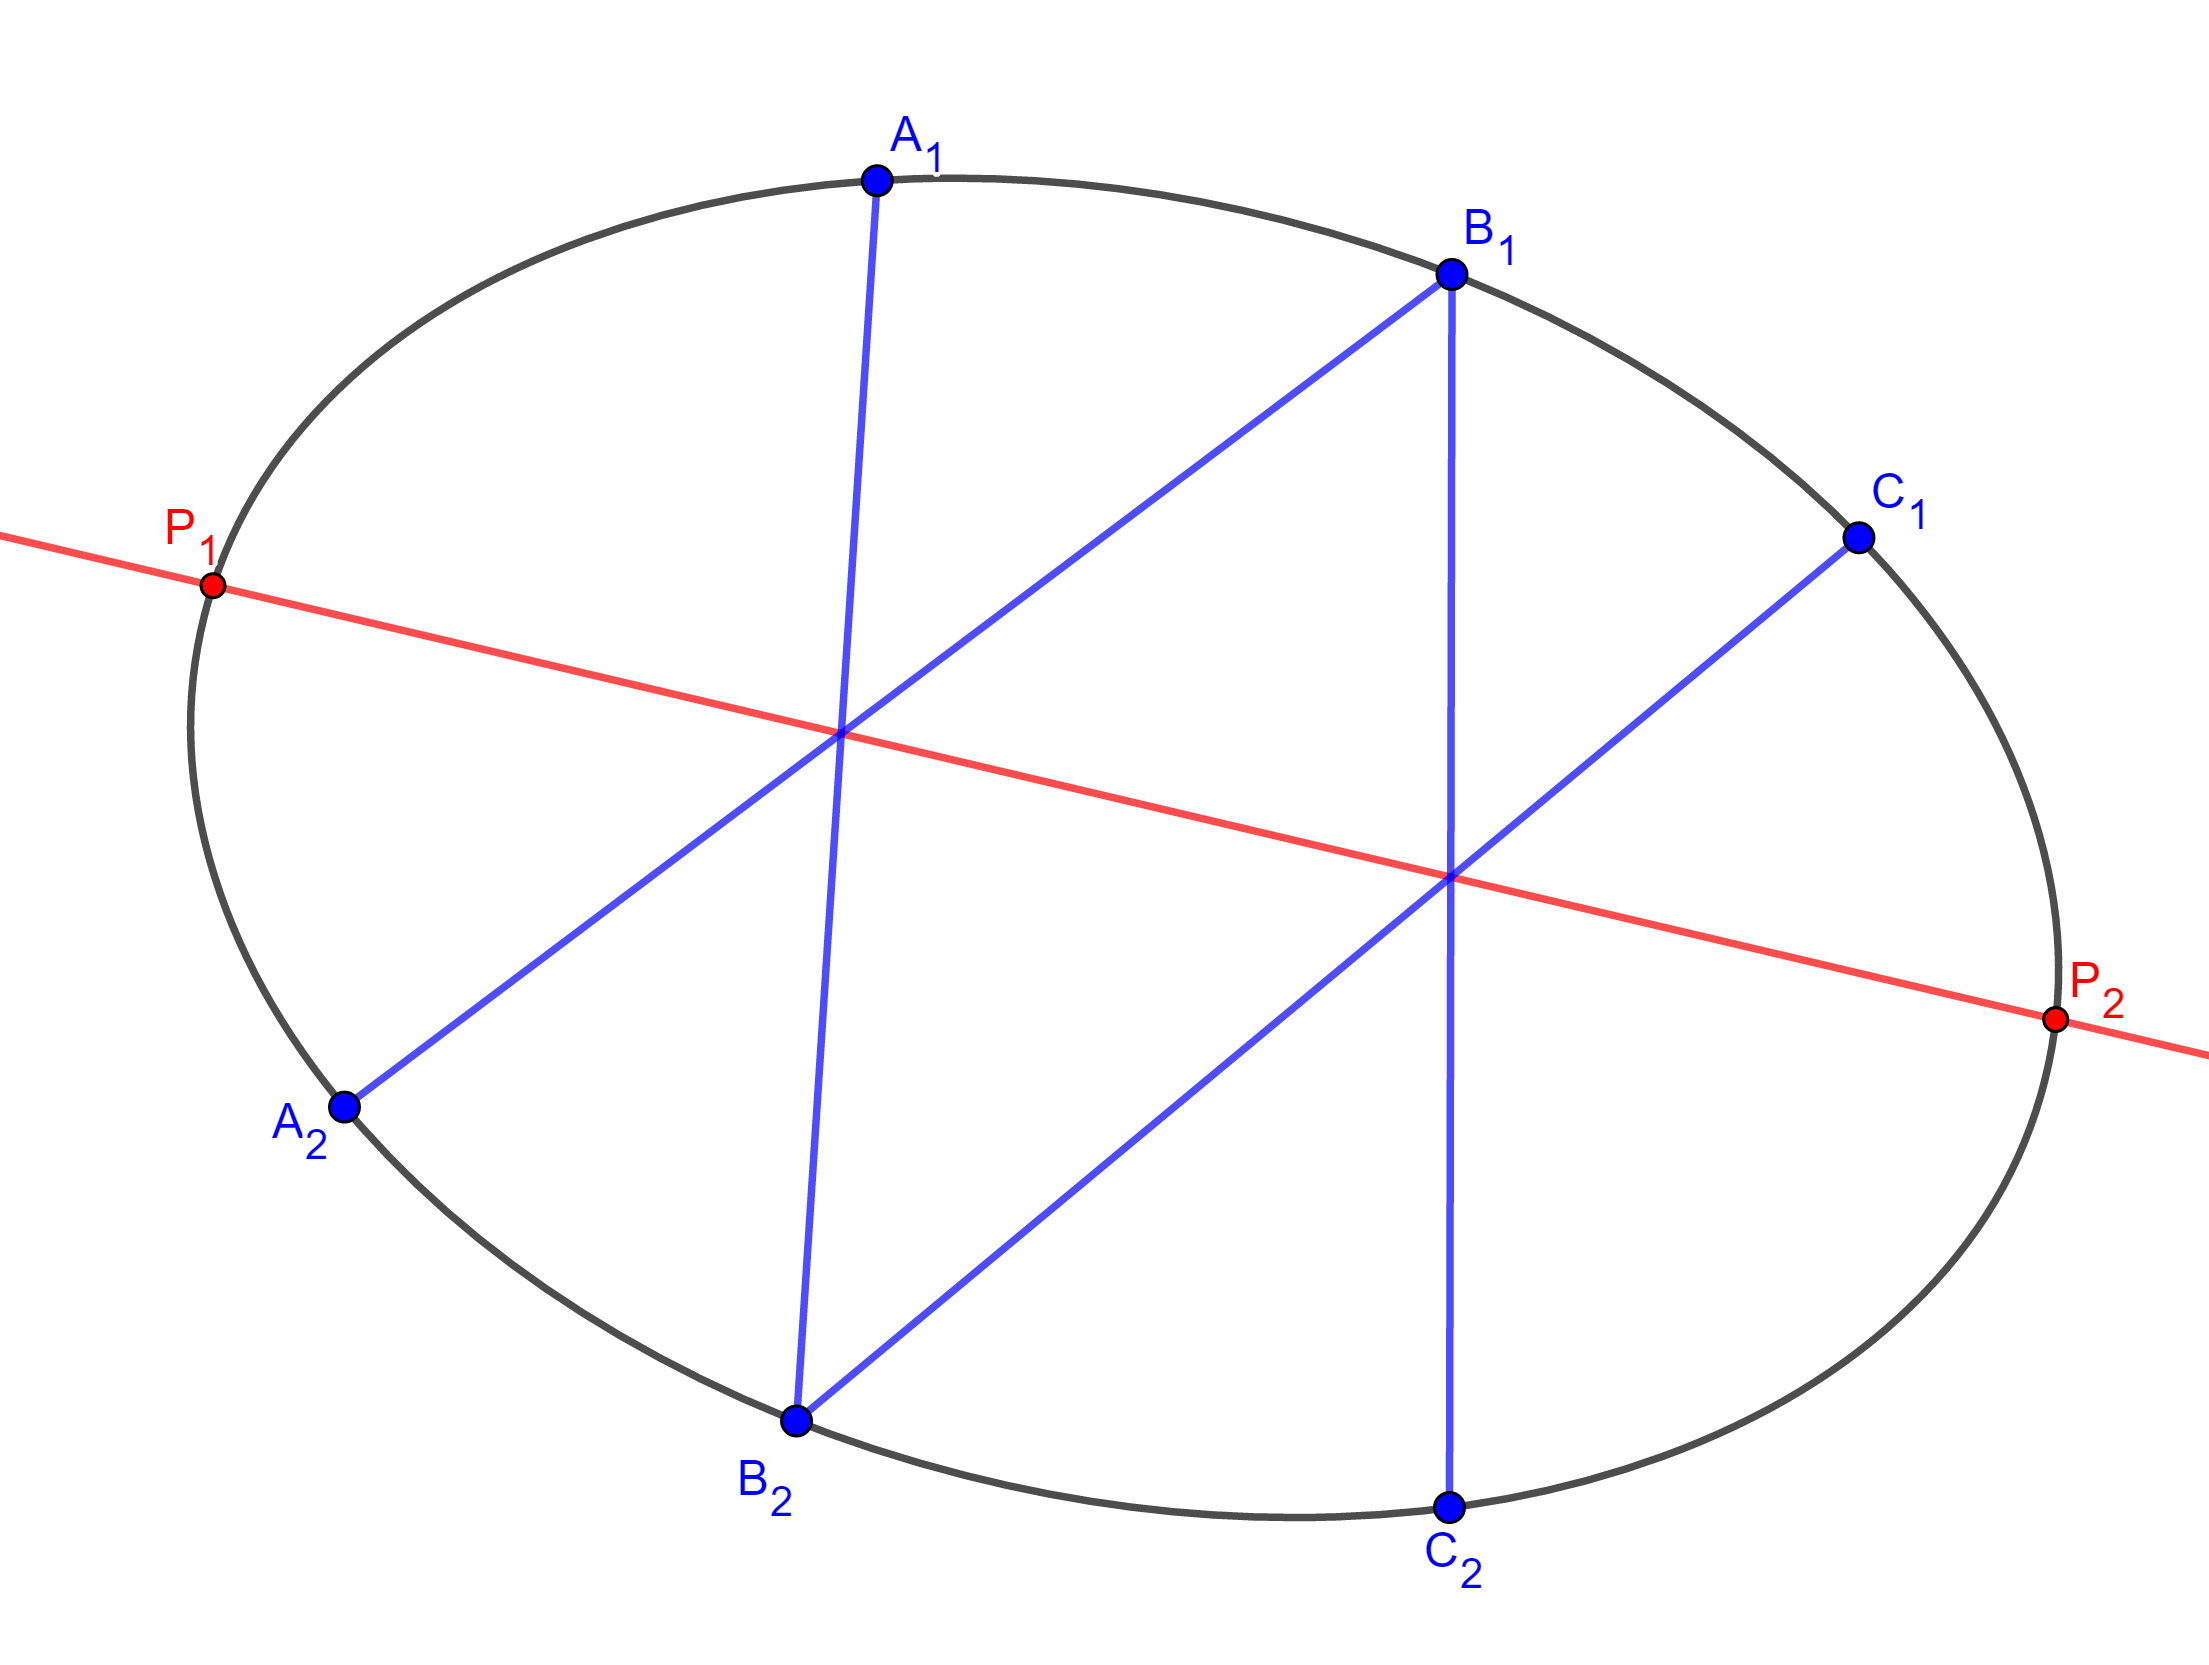
\includegraphics[width=500px]{pic16.png}
\end{figure}
\textbf{Определение предела по Гейне:}
 
     Пусть  $c, d\in\re\cup\{\infty, +\infty, -\infty\}$. Тогда $\lim\limits_{x\to c\pm 0} f(x) = d$, если для любой последовательности $\{x_n\}$ с условием $\Forall n\; x_n \neq c$ и $\lim\limits_{n\to\infty} x_n = c$ выполнено $\lim\limits_{n\to\infty} f(x_n) = d$.\\\\
     
%tic17
\section*{Вопрос 17}
\begin{center}
  Свойства пределов функций: арифметические и связанные с неравенствами или сохранение знака нестрогого неравентсва при переходе к пределу(с доказательством одного из них) :$\lim(f(x)+g(x)), \lim(f(x)\cdot g(x))$
\end{center}
\subsection*{Ответ:}
\textbf{Доказательство предела суммы (или разности):}\\
Пусть $s(x)=f(x)+g(x)$
Используя арифметические свойства пределов последовательностей, имеем:
$\lim\limits_{x\to \infty} s(X_n) = \lim\limits_{x\to \infty} (f(X_n)\pm g(X_n))  = \lim\limits_{x\to \infty} f(X_n) \pm \lim\limits_{x\to \infty} g(X_n) = a \pm b$
Поскольку $\{X_n\}$ есть произвольная последовательность, сходящаяся к $x_0$ и элементы которой принадлежат окрестности $\stackrel{\circ}{U}(x_0)$ , то, согласно определению предела функции по Гейне,$\lim\limits_{x\to x_0} s(x) = a \pm b, \lim\limits_{x\to x_0} (f(x)\pm g(x)) = a \pm b$
\\
\textbf{Доказательство предела произведения:}\\
Пусть $p(x)=f(x)\cdot g(x)$, тогда $\lim\limits_{x\to \infty} p(X_n) = \lim\limits_{x\to \infty} (f(X_n) \cdot g(X_n)) = \lim\limits_{x\to \infty} f(X_n) \cdot \lim\limits_{x\to \infty} g(X_n) = a \cdot b$.
Поскольку $\{X_n\}$ есть произвольная последовательность, сходящаяся к $x_0$ и элементы которой принадлежат окрестности $\stackrel{\circ}{U}(x_0)$ , то, согласно определению предела функции по Гейне,$\lim\limits_{x\to \infty} p(x) = a \cdot b$,
$\lim\limits_{x\to \infty} (f(x) \cdot g(x)) = a \cdot b$\\
\textbf{Сохранение знака нестрогого неравентсва при переходе к пределу:}
\begin{center}
  Если существуют конечные пределы: $\lim\limits_{x \to x_0} f_1(x) = a_1$ и $\lim\limits_{x \to x_0} f_2(x) = a_2$ и на некоторой проколотой окрестности $\stackrel{\circ}{U}(x_0)$ точки $x_0$ $f_1(x) \leq f_2(x)$, то $a_1 \leq a_2$
\end{center}
\textbf{Доказательство сохранения знака нестрогого неравентсва при переходе к пределу:}\\
Пусть $\{X_n\}$ есть произвольная последовательность, сходящаяся к $x_0$: $\lim\limits_{n \to \infty} X_n = x_0$. И пусть ее элементы принадлежат проколотой окрестности точки , на которой выполняется неравенство $f_1(x) \leq f_2(x)$.\\
Рассмотрим последовательности $\{f_1(x)\}$ и $\{f_2(x)\}$.
Поскольку $\lim\limits_{x \to x_0} f_1(x) = a_1$
и $\lim\limits_{x \to x_0} f_2(x) = a_2$
, то согласно определению предела функции по Гейне, эти последовательности имеют пределы:  $\lim\limits_{n \to \infty} f_1(X_n) = a_1$, $\lim\limits_{n \to \infty} f_2(X_n) = a_2$\\
Поскольку $f_1(x) \leq f_2(x)$ , то их элементы связаны неравенствами:
$f_1(X_n) \leq f_2(X_n)$. Тогда $\lim\limits_{n \to \infty} f_1(X_n) \leq \lim\limits_{n \to \infty} f_2(X_n)$\\ отсюда $a_1 \leq a_2$
%tic18
\section*{Вопрос 18}
\begin{center}
  Первый и второй замечательный пределы(первый с доказательством)
\end{center}
\subsection*{Ответ:}
\textbf{Второй замечательный предел:}\\
$\lim\limits_{x \to \infty} (1 + \frac{1}{x})^x = e$\\
\textbf{Первый замечательный предел:}\\
$\lim\limits_{x \to 0} \frac{\sin x}{x} = 1$\\
\textbf{Доказательство:}\\
Нарисуйте себе тригонометрическую окружность и отметьте там точку $x \in \left(0; \dfrac{\pi}{2}\right)$. Теперь исходя из этой же тригонометрической окружности видно: $\sin x < x < \tg x$. \\
Разделим на $\sin x$, зная, что он больше нуля для такого $x$: \\
$1 < \dfrac{x}{\sin x} < \dfrac{1}{\cos x} \Leftrightarrow 1 > \dfrac{\sin x}{x} > \cos x$. По лемме о двух милионерах получим $\dfrac{\sin x}{x} \to 1$ при $x \to 0$.
 
%tic19
\section*{Вопрос 19}
\begin{center}
  Определение эквивалентных функций. О-символика(определения "О большого" и
  "о малого")
\end{center}
\subsection*{Ответ:}
\textbf{Определение эквивалентных функций:} $f(x)$ и $g(x)$ называются эквивалентными при $x \to c$ если $\lim\limits_{x \to c} \frac{f(x)}{g(x)} = 1$ обозначается как $f \sim g$\\
\textbf{О-символика определение:}\\
Говорят, что $f(x) = O(g(x))$ $(f(x))$ есть (\underline{\underline{o}}) О большое от $g(x)$
при $x \to c$, если в некоторой проколотой окрестности точки $x = c, (f(x) \leq a(g(x))$
для некоторой константы a. Если $c = \infty$, то вместо проколотой окрестности в определении
надо брать $(-\infty,-\delta) \vee (\delta, +\infty)$ \\
Говорят, что $f(x) = o(g(x))$,\; $f(x)$ есть ($\bar{\bar{o}}$)\; о малое от $g(x)$ при $x \to c$ если $\lim\limits_{x \to c} \frac{f(x)}{g(x)} = 0$ по другому
$f(x) = g(x) \cdot d(x)$, где $d(x) \to 0$ при $x \to c$
%tic20
\section*{Вопрос 20}
\begin{center}
  Стандартные эквивалентности (с выводом каких-нибудь трех из них)
\end{center}
\subsection*{Ответ:}
\begin{center}
При $x \to 0$
  $(1 + x)^p \sim 1 + p \cdot x$\\
  $e^x \sim 1 + x$\\
  $\ln(1+x) \sim x$\\
  $\sin x \sim \arcsin x \sim \tg x \sim x$\\
  $\cos x \sim 1 - \frac{x^2}{2}$\\
\end{center}
\textbf{Докажем, что $\tg x \sim x$:}\\
$\lim\limits_{x \to 0} \frac{\tg x}{x} = \lim\limits_{x \to 0} \frac{\frac{\sin x}{x}}{\cos x} =
\frac{\lim\limits_{x \to 0} \frac{\sin x}{x}}{\lim\limits_{x \to 0} \cos x} = \frac{1}{1} = 1$\newline
\textbf{Докажем, что $\cos x \sim 1 - \frac{x^2}{2}$:}\\
$\cos^2 x = 1 - \sin^2 x, \; \cos x = \sqrt{1 - \sin^2 x} \sim \sqrt{1 - x^2} \sim 1 - \frac{x^2}{2}$\newline
\textbf{Докажем, что $\sin x \sim x$:}\newline
(Доказывая первый замечательный предел, мы доказали, что $\sin x \sim x$\\
 
%tic21
\section{Определение непрерывности по Коши и Гейне. Классификация точек разрыва функций}
   
   \textbf{\underline{Определение:}} Функция $f(x)$ непрерывна в точке $x_0$, если $\lim\limits_{x\to x_0} f(x) = f(x_0)$.\newline
   Пусть $f(x)$ определена на $A\subseteq\re$.\newline
   \subsection*{\underline{Непрерывность по Коши}:}
       $\Forall\eps > 0\;\Exists\delta\;\Forall x\in\;(x_0 - \delta; x_0 + \delta)\cap A\;\abs{f(x) - f(x_0)} < \eps$.
   \subsection*{\underline{Непрерывность по Гейне}:}
       Для любой последовательности $x_n\colon \lim\limits_{n\to\infty} x_n = x_0$ верно, что $\lim\limits_{n\to\infty} f(x_n) = f(x_0)$.\newline
   \textbf{\underline{Определение:}} Функция непрерывна на некотором множества $A$ (на котором она опредедена), если $f(x)$ непрерывна в $x_0 \;\Forall x_0\in A$.\newline
   Функция непрерывна, если $\lim\limits_{n\to\infty} f(x_n) = f\left(\lim\limits_{n\to\infty} x_n\right)$. То есть непрерывные функции можно менять местами с пределами.\newline
   
   \subsection*{\underline{Точки разрыва}:}
   Если $f(x)$ не обладает свойством непрерывности в точке $x_0$, то $x_0$ - точка разрыва. Принята следующая классификация точек разрыва:
   \begin{enumerate}
       \item Если $\lim\limits_{x\to x_0 + 0} f(x)$ и $\lim\limits_{x\to x_0 - 0} f(x)$ существуют, конечны и равны, то $x_0$ называется точкой устранимого разрыва. Можно положить $f(x_0) := \lim\limits_{x\to x_0} f(x)$. Тогда $f(x)$ становится непрерывной в $x_0$.\newline
       \textbf{\underline{Пример}}: Рассмотрим функцию $f(x) = \abs{sign(x)}$. $f(0) \neq \lim\limits_{x\to 0 - 0} = \lim\limits_{x\to 0 + 0} = 1$.
       
       \item Если оба односторонних предела существуют, конечны, но не равны, то разрыв называется разрывом первого рода. Для такого разрыва определен скачок функции $\Delta_{x_0} f = \lim\limits_{x\to x_0 + 0} f(x) - \lim\limits_{x\to x_0 - 0} f(x)$\newline
       \textbf{\underline{Пример}}: Рассмотрим функцию $f(x) = sign(x)$. $f(0) \neq \lim\limits_{x\to 0 - 0} \neq \lim\limits_{x\to 0 + 0}; d = 2$.
       
       \item Если не существует или существует бесконечный хотя бы один односторонний предел, это разрыв 2 рода (то есть все, что не вышеперечисленное /shrug).\newline
       \textbf{\underline{Пример}}: $f(x) = \dfrac{1}{x}$.
   \end{enumerate}
   
\bigskip\bigskip
%tic22
\section{Свойства непрерывных функций}
   \subsection*{Теорема о сохранении знака}
       \textbf{\underline{Утверждение}}: Если $f(x)$ непрерывна в $x_0$ и $f(x_0)\neq 0$, то в некоторой окрестности $x_0$ $f(x)$ имеет тот же знак, что и $f(x_0)$.\newline
       \textbf{\underline{Доказательство}}:
           Предположим, что $f(x) := d > 0$. \newline
           Из непрерывности по Коши: $\Forall\eps > 0\;\Exists\delta\;\Forall x\in\;(x_0 - \delta; x_0 + \delta);\abs{f(x) - d} < \eps$.\newline
           Возьмем $\eps = \nicefrac{d}{2}$. Получим $\abs{f(x) - d} < \nicefrac{d}{2} \Leftrightarrow -\nicefrac{d}{2} < f(x) - d < \nicefrac{d}{2} \Leftrightarrow \nicefrac{d}{2} < f(x) < \nicefrac{3d}{2}, d > 0 \Rightarrow f(x) > 0$.
   \subsection*{Арифметические}
       Если $f(x)$ и $g(x)$ непрерывны в $x_0$, то $f(x)\pm g(x), f(x)\cdot g(x)$ и $\dfrac{f(x)}{g(x)}$ (при $g(x)\neq 0$) непрерывны в $x_0$. Это следует из арифметических свойств пределов, если воспользоваться $\lim\limits_{x\to c} f(x) = f(c)$
       \textbf{\underline{Замечание}}:
           Исходя из теоремы о сохранении знака, в случае частного функций требуется дополнительно проверить, что в некоторой окрестности $x_0$ $g(x) \neq 0$.
           
   \subsection*{Непрерывность композиции}
       \textbf{\underline{Утверждение}}: Пусть $g(x)$ непрерывна в $x_0$, а $f(y)$ непрерывна в $y_0 = g(x_0)$, тогда $f\circ g = f(g(x))$ непрерывна в $x_0$. \newline
       \textbf{\underline{Доказательство}}: Пусть $x\to x_0$. Тогда $g(x_n)\to g(x_0) = y_0$ (по непрерывности $g(x)$). \newline
       Тогда $f(g(x_n))\to f(y_0)$ (по непрерывности $f(y)$) \newline
       Написанное верно $\Forall x_n\to x_0$, значит $f(g(x))$ непрерывна в $x_0$.\newline\newline
       \textbf{\underline{Можно проще}}: $\lim\limits_{n\to\infty} f(g(x_n)) = f(\lim\limits_{n\to\infty} g(x_n)) = f(g(\lim\limits_{n\to\infty} x_n)) = f(g(x_0))$. Выполняется непрерывность по Гейне, утверждение доказано.
       
\bigskip\bigskip
%tic23
\section{Теорема Вейерштрасса о достижимости непрерывной функции точной верхней и нижней граней на отрезке}
\textbf{\underline{Определение:}} Говорят, что $f(x)$ достигает своей точной верхней грани на множества $A$, если $\Exists x_0\in A\colon f(x_0) = \sup\limits_{x\in A} f(x)$ (Аналогично с нижней).
\textbf{\underline{Определение:}} Говорят, что $f(x)$ непрерывна на $A\in\re$, если $f(x)$ непрерывна в любой точке $x_0\in A$.\newline
\textbf{\underline{Обозначение:}} $C(A)$ -- множество всех функций, непрерывных на $A$. \newline
 
\subsection*{Теорема Вейерштрасса}
\textbf{\underline{Утверждение}}: Если $f(x)\in C([a, b])$, то $f(x)$ ограничена и принимает наибольшее и наименьшее значение.
\textbf{\underline{Доказательство}}: Докажем ограниченность сверху и достижимость супремума.
\begin{enumerate}
   \item \textbf{Ограниченность от противного}. Допустим, что $f(x)$ не ограничена сверху. Значит, $\Forall n\in\n\Exists x_n\in [a, b]\; f(x_n)\geq n$. \newline
   Согласно теореме Больцано-Вейерштрасса, $\Exists$ сходящаяся подпоследовательность $\{x_{n_k}\}_{k = 1}^{\infty}$. Пусть $c := \lim\limits_{k\to\infty} {x_{n_k}}$. \newline
   $x_{n_k}\to c\in [a, b] \xRightarrow[\text{по непрервыности в точке}\; c]{} f(x_{n_k})\to f(c)\in\re$. \newline
   Получаем $f(x_{n_k}) \geq n_k \Rightarrow \lim\limits_{k\to\infty} f(x_{n_k}) = +\infty$ и $\lim\limits_{k\to\infty} f(x_{n_k}) = f(c)\in\re$ -- противоречие.
   \item \textbf{Достижимость супремума}. Пусть $s := \sup\limits_{x\in [a, b]} \{f(x)\}$. Так как $s$ -- это т.в.г., то в $x_n$ можно выделить $x_{n_k}$, причем $x_{n_k}\to c\in [a, b]$. $f$ непрерывна на $[a, b]$, тогда $f(c) = \lim\limits_{x\to \infty} f(x_{n_k}) = \lim\limits_{x\to \infty} f(x_n) \;(по\;Больц.-В.) = s = f(c) = f(x_{n_k})$. Значит, супремум достигается в точке $c$. Аналогично делаем для инфимума.
\end{enumerate}
 
\bigskip\bigskip
%tic24
\section{Теорема Коши о промежуточном значении. Метод деления пополам для поиска корней уравнения}
\textbf{\underline{Утверждение}}: Пусть $f(x)\in C([a, b])$. Тогда для любого числа $d$ между $f(a)$ и $f(b)$ $\Exists x_0\in [a, b]\colon f(x_0) = d$.
\textbf{\underline{Доказательство}}: Для определенности, пусть $f(a) \leq d \leq f(b)$.\newline
Разобьем $[a, b]$ пополам и выберем ту половину $[a_1, b_1]$, для которой выполнено $f(a_1)\leq d\leq f(b_1)$.\newline
Повторим операцию: делим $[a_1, b_1]$ пополам и обозначим за $[a_2, b_2]$ ту половину, для которой $f(a_2) \leq d \leq f(b_2)$.\newline
Действуя аналогично, получаем последовательность отрезков $[a_n, b_n]$, таких, что $f(a_n) \leq d \leq f(b_n)$. Заметим, что последовательность вложенная и стягивающаяся. Значит, $\Exists ! c\in [a_n, b_n]$. В частности: $a_n\to c, b_n\to c$ при $n\to\infty \Rightarrow f(a_n)\to f(c)$ и $f(b_n)\to f(c)$ (следует из непрерывности). \newline
Итого получаем из сходимости, что $f(a_n) \leq d \leq f(b_n) \Leftrightarrow f(c) \leq d \leq f(c) \Rightarrow f(c) = d$.\newline
\textbf{\underline{Следствие}}: Если $f\in C([a, b])$ и $f(a)\cdot f(b) \leq 0$, то $\Exists c\in [a, b]$, такое что $f(c) = 0$. \newline
То есть это означает по сути-то, что $f$ еще и монотонна, короче, корни ищем бинпоиском, ну вы поняли, окда.
 
\bigskip\bigskip
%tic25
\section{Теорема о существовании обратной функции}
\textbf{\underline{Утверждение}}: Пусть $f(x)\in C([a, b])$ и строго монотонна на $[a, b]$. Тогда у $f$ существует обратная функция $g$, заданная на $[A, B] = [f(a), f(b)]$ и $g$ -- непрерывна и монотонна на $[A, B]$.
\textbf{\underline{Доказательство}}: $f(g(x)) = x$ (ну потому что обратная функция)\newline
$\Forall d\in [A, B] \Exists c\in [a, b]$, такое что $f(c) = d$ (по теореме Коши о промежуточном значении). Такое $c$ еще и единственно, потому что $f$ монотонна.\newline
Тогда положим $g(d) := c$. Имеем $f(g(d)) = f(c) = d$.
%TODO: че бля за свойства????
 
 
\bigskip\bigskip
%tic26
\section{Производная (приращение аргумента, функции, геометрический смысл). Уравнение прямой, касательной к графику дифференцируемой функции. Односторонние производные. Пример непрерывной функции, не имеющей производной в заданной точке.}
\subsection*{Производная и ее геометрический смысл}
\textbf{\underline{Определение}}: Пусть $f(x)$ определена в некоторой окрестности точки $x_0\in\re$. Тогда предел $\lim\limits_{x\to x_0} \dfrac{f(x) - f(x_0)}{x - x_0}$, если он существует и конечен, называется производной $f(x)$ в точке $x_0$ и обозначется $f'(x_0)$. \\
\textbf{\underline{Обозначение}}: \\
$\Delta x := x - x_0$ -- приращение аргумента функции. \\
$\Delta f := f(x_0 + \Delta x) - f(x_0)$ -- приращении функции.\\
Тогда $f'(x_0) = \lim\limits_{\Delta x\to 0} \frac{\Delta f}{\Delta x}$. \\
\textbf{\underline{Геометрический смысл}}: $\frac{\Delta f}{\Delta x}$ -- тангенс угла наклона секущей.
\begin{figure}[H]
%   \includegraphics[width=128px]{pict003.png}
\end{figure}
   
   
При $\Delta x\to 0$ секущая -- это касательная в $x_0$. Таким образом, касательная к графику функции $y = f(x)$ в точке $A$ - это предельное положение секущей $AB$ при $B\to A$ (смотри рисунок :cool\_story\_bob:)
\begin{figure}[H]
%   \includegraphics[width=128px]{pict006.png}
\end{figure}
   
Отсюда достаточно простот выводится уравнение касательной. Очевидно, что ее вид будет $y = f'(x_0)\cdot x + b$. Из касания следует: $f(x_0) = f'(x_0)\cdot x_0 + b \Leftrightarrow b = f(x_0) - f'(x_0)\cdot x_0$.\\
Подставим в исходное равенство: $y = f'(x_0)\cdot x + f(x_0) - f'(x_0)\cdot x_0 = f'(x_0)(x - x_0) + f(x)$ -- касательная к $f(x)$ в точке $x_0$. \\
\subsection*{Односторонняя производная}
\textbf{\underline{Определение}}: Левая (правая) производная функции $f(x)$ -- это её левый (правый) предел $\lim\limits_{\Delta x\to 0\mp 0} \frac{\Delta f}{\Delta x}$. \\
\textbf{\underline{Обозначение}}: $f'_{-}(x)$ и $f'_{+}(x)$ соотвественно.\\
\textbf{\underline{Пример непрерывной функции, не дифференцируемой в заданной точке}}: $f(x) = \abs{x}$ не дифференцируема в точке $x = 0$.
 
\bigskip\bigskip
%tic27
\section{Связь между существованием производной и непрерывностью функции в данной точке}
Из существования $\lim\limits_{\Delta x\to 0} \frac{\Delta f}{\Delta x}$ следует, что при $\Delta x\to 0 \Delta f\to 0$, что фактически означает непрерывность в $x_0$. В обратную сторону работает аналогично. (Примечание: пните, если тут еще что-то нужно добавить, автор долбоеб).
 
\subsection*{Арифметические свойства производных}
\begin{enumerate}
   \item $(f\pm g)'(x_0) = f'(x_0)\pm g'(x_0)$. \\
   \textbf{\underline{Доказательство}}: Очевидно. \\
   Tank mode on: $(f\pm g)'(x_0) = \frac{(f(x_0 + \Delta x) - f(x_0)) \pm (g(x_0 + \Delta x) - g(x_0))}{\Delta x} = \frac{f(x_0 + \Delta x) - f(x_0)}{\Delta x} \pm  \frac{g(x_0 + \Delta x) - g{x_0}}{\Delta x} = f'(x_0) \pm g'(x_0)$. Tank mode off.
   
   \item $(fg)'(x_0) = f'(x_0)g(x_0) + f(x_0)g'(x_0)$. \\
   \textbf{\underline{Доказательство}}: \\
   $(fg)'(x_0) = \lim\limits_{\Delta x\to 0} \dfrac{f(x_0 + \Delta x)g(x_0 + \Delta x) - f(x_0)g(x_0)}{\Delta x} = \\
   \lim\limits_{x\to 0} \dfrac{f(x_0 + \Delta x)g(x_0 + \Delta x) - \left[f(x_0)g(x_0 + \Delta x) - f(x_0)g(x_0 + \Delta x) \right] - f(x_0)g(x_0)}{\Delta x} = \lim\limits_{x\to 0} \dfrac{f(x_0 + \Delta x) - f(x_0)}{\Delta x}\cdot g(x_0 + \Delta x) + \lim\limits_{x\to 0} \dfrac{g(x_0 + \Delta x) - g(x_0)}{\Delta x}\cdot f(x_0) = f'(x_0)g(x_0) + f(x_0)g'(x_0)$.
   
   \item $\left(\dfrac{1}{g}\right)'(x_0) = \dfrac{-g'(x_0)}{g^2(x_0)}$. \\
   \textbf{\underline{Доказательство}}: \\
   $\left(\dfrac{1}{g}\right)'(x_0) = \lim\limits_{\Delta x\to 0} \dfrac{\dfrac{1}{g(x_0 + \Delta x)} - \dfrac{1}{g(x_0)}}{\Delta x} = \lim\limits_{\Delta x\to 0} \dfrac{-(g(x_0 + \Delta x) - g(x_0))}{\Delta x\cdot g(x_0 + \Delta x)g(x_0)} = \\ \lim\limits_{\Delta x\to 0} \dfrac{-(g(x_0 + \Delta x) - g(x_0))}{\Delta x} \cdot \lim\limits_{\Delta x\to 0} \dfrac{1}{g(x_0 + \Delta x)g(x_0)} = \dfrac{-g'(x_0)}{g^2(x_0)}$.
   
   \item $\left(\dfrac{f}{g}\right)'(x_0) = \dfrac{f'(x_0)g(x_0) - g'(x_0)f(x_0)}{g^2(x_0)} = \left(f\cdot \dfrac{1}{g}\right)' = f'\cdot\dfrac{1}{g} + f\cdot\left(\dfrac{1}{g}\right)'$ -- дальше просто воспользоваться предыдущим свойством.
\end{enumerate}
 
\bigskip\bigskip
%tic28
\section{Производная композиции функций и производная обратной функции}
\subsection*{Производная композиции}
\textbf{\underline{Утверждение}}: $(f(g(x)))' = f'(g(x))\cdot g'(x)$, если существует $g'(x)$ и $f'$ в точке $g(x)$. \\ \\
\textbf{\underline{Доказательство}}: \\
$\lim\limits_{\Delta x\to 0} \dfrac{f(g(x_0 + \Delta x)) - f(g(x_0))}{\Delta x} = \lim\limits_{\Delta x\to 0} \dfrac{f(g(x_0 + \Delta x)) - f(g(x_0))}{g(x_0 + \Delta x) - g(x_0)}\cdot\dfrac{g(x_0 + \Delta x) - g(x_0)}{\Delta x} = \\ \begin{bmatrix} g(x_0) = y_0, g(x_0 + \Delta x) = y_0 + \Delta y \\ \Delta x\to 0 \Rightarrow \Delta y\to 0,\text{ т.к. } g \text{ непрерывна в } x_0 \end{bmatrix} = \lim\limits_{\Delta y\to 0} \dfrac{f(y_0 + \Delta y) - f(y_0)}{\Delta y} \cdot \lim\limits_{\Delta x\to 0}\dfrac{g(x_0 + \Delta x) - g(x_0)}{\Delta x} = f'(y_0)\cdot g'(x_0) = f'(g(x_0))\cdot g'(x_0)$.
 
 
\subsection*{Производная обратной функции}
\textbf{\underline{Утверждение}}: Пусть $y = f(x)$ непрерывна и строго монотонна в некоторой окрестности точки $x_0\in\re$ и $f(x_0) \neq 0$. Тогда обратная функция $x = g(y) = f^{-1}(y)$ имеет производную в точке $f(x_0)$ и $g'(y_0) = \dfrac{1}{f'(x_0)}$.\\
\textbf{\underline{Доказательство}}: \\
$\lim\limits_{\Delta y\to 0} \dfrac{g(y_0 + \Delta x) - g(y_0)}{\Delta y} = \begin{bmatrix} \Delta y = \Delta f = f(x_0 + \Delta x) - f(x_0) \\ g(y_0) = x_0 \\ g(y_0 + \Delta y) = x_0 + \Delta x \\ \Delta x\to 0 \Leftrightarrow \Delta y\to 0 \text{ из непрерывности } f\; и\; g \end{bmatrix} = \lim\limits_{\Delta x\to 0} \dfrac{\Delta x}{f(x_0 + \Delta x) - f(x_0)} = \\ \dfrac{1}{\lim\limits_{\Delta x\to 0} \dfrac{f(x_0 + \Delta x) - f(x_0)}{\Delta x}} = \dfrac{1}{f'(x_0)}$. \\
\textbf{\underline{Важное следствие}}:
$(f^{-1})'(y_0) = \dfrac{1}{f'(f^{-1}(y_0))}$ (потому что $x_0 = f^{-1}(y_0)$).
Это очень полезно при нахождении производных. Например, пусть надо найти производную $(\arcsin{y})'$. Тогда $(\arcsin{y})' = \dfrac{1}{\sin'(\arcsin y)} = \dfrac{1}{\cos(\arcsin y)}$. Дальше тупо выразить косинус через синус.
 
\bigskip\bigskip
%tic29
\section{Вывод табличных производных}
 
\subsection{$f(x) = \log_a x$}
%$(\log_a x)' = \lim\limits_{\Delta x\to 0} \dfrac{\log_a (x + \Delta) - \log_a x}{\Delta x} = \lim\limits_{\Delta x\to 0}\dfrac{\log_a\dfrac{x + \Delta x}{x}}{\Delta x} = \lim\limits_{\Delta x\to 0}\dfrac{1}{\Delta x}\cdot \log_a(1 + \dfrac{\Delta x}{x}) = \\ \lim\limits_{\Delta x\to 0} \log_a (1 + \dfrac{\Delta x}{x})^{\nicefrac{1}{\Delta x}} = \lim\limits_{\Delta x\to 0} \log_a \left(1 + \dfrac{\Delta x}{x}\right)^{\frac{x}{x\cdot\Delta x}} = \dfrac{1}{x}\log_a \lim\limits_{\Delta x\to 0} \left(1 + \dfrac{\Delta x}{x}\right)^{\frac{x}{\Delta x}} = \dfrac{1}{x}\cdot\log_a \e = \dfrac{1}{x}\cdot\dfrac{\ln e}{\ln a} = \dfrac{1}{x\ln a}$. \\
\subsection{$f(x) = x^a$}
Воспользуемся предыдущей формулой. \\
$y = x^a \Leftrightarrow \ln y = \ln x^a \Leftrightarrow \ln y = a\cdot\ln x$. \\
$(\ln y)' = (a\cdot\ln x)'$ \\
$\dfrac{1}{y}\cdot y' = a\cdot\dfrac{1}{x} \Rightarrow y' = a\dfrac{y}{x} = p\cdot\dfrac{x^a}{x} = p\cdot x^{p - 1}$.\\
Осталось доказать для $x < 0$. Это возможно только для $a\; mod\; 2 = 1$. \\
$y(x) = -y(-x)$
$y'(x) = (-(-x)^a)' = -((-x)^a)' = -a\cdot (-x)^{a - 1}\cdot (-x)' = a\cdot(-x)^{a - 1} = a\cdot x^{a - 1}$.
 
\subsection{$f(x) = a^x$}
$f'(x_0) = \lim\limits_{\Delta x\to 0}\dfrac{a^{x_0 + \Delta x} - a^{x_0}}{\Delta x} = \lim\limits_{\Delta x\to 0}\dfrac{a^{x_0}(a^{\Delta x} - 1)}{\Delta x}$. Получили неопределенность, сасатб /shrug. \\
Пусть $z = a^{\Delta x} - 1 \Rightarrow z + 1 = a^{\Delta x} \Rightarrow \Delta x = \log_a (z + 1) = \dfrac{\ln(z + 1)}{\ln a}$. \\
$\lim\limits_{\Delta x\to 0}\dfrac{a^{x_0}(a^{\Delta x} - 1)}{\Delta x} = a^{x_0}\cdot\lim\limits_{\Delta z\to 0}\dfrac{z}{\dfrac{\ln(z + 1)}{\ln a}} = a^{x_0}\cdot\ln a\cdot\lim\limits_{\Delta z\to 0}\dfrac{z}{\ln(z + 1)} = a^{x_0}\cdot\ln a\cdot\lim\limits_{\Delta z\to 0}\dfrac{1}{\dfrac{1}{z}\ln(z + 1)} = a^{x_0}\cdot\ln a\cdot\lim\limits_{\Delta z\to 0}\dfrac{1}{\ln(z + 1)^{\nicefrac{1}{z}}} = a^{x_0}\cdot\ln a\cdot\dfrac{1}{\ln e} = a^{x_0}\ln a$.\\ \\ \\
\subsection{$f(x) = \sin x$}
$f'(x_0) = \lim\limits_{\Delta x\to 0}\dfrac{\sin(x_0 + \Delta x) - \sin\Delta x_0}{\Delta x} = [\textrm{по формуле разности синусов}] = \lim\limits_{\Delta x\to 0} \dfrac{\sin\dfrac{\Delta x}{2}\cos\left(x_0 + \dfrac{\Delta x}{2}\right)}{\dfrac{\Delta x}{2}} = \cos x_0$.
 
\subsection{$f(x) = \cos x$}
$f'(x_0) = \lim\limits_{\Delta x\to 0} \dfrac{\cos(x_0 + \Delta x) - \cos x_0}{\Delta x} = \lim\limits_{\Delta x\to 0} \dfrac{-sin(x_0 + \dfrac{\Delta x}{2})\sin\left(\dfrac{\Delta x}{2}\right)}{\dfrac{\Delta x
}{2}} = -sin(x_0)$
 
\subsection{$f(x) = \tg x$}
$f'(x_0) = \left(\dfrac{\sin x_0}{\cos x_0}\right)' = \dfrac{\cos^2(x_0) + \sin^2(x_0)}{\cos^2(x_0)} = \dfrac{1}{\cos^2 x}$.
 
\subsection{$f(x) = \arcsin x$}
$f'(x_0) = \dfrac{1}{\sin'(\arcsin (x_0))} = \dfrac{1}{\cos(\arcsin x_0)} = \dfrac{1}{\sqrt{1 - \sin^2(\arcsin x_0))}} = \dfrac{1}{\sqrt{1 - x_0^2}}$.
 
\subsection{$f(x) = \arctg x$}
 
$f'(x_0) = \dfrac{1}{\tg'(\arctg(x_0))} = \cos^2(\arctg(x_0)))$. \\
Положим $y = \arctg(x_0))$. \\
$\dfrac{1}{\cos^2(y)} = \dfrac{\sin^2 y + \cos^2 y}{\cos^2(y)} = 1 + \tg^2(y) = 1 + x^2$. \\
Тогда $\dfrac{1}{\tg'(\arctg(x_0))} = \cos^2(\arctg(x_0))) = \dfrac{1}{1 + x^2}$.
 
\bigskip\bigskip
%tic30
\section{Дифференциал: определение, геометрический смысл, арифметические свойства. Инвариантность формы первого дифференциала}
 
\textbf{\underline{Определение}}: Пусть $f(x)$ определена в окрестности точки $x_0\in\re$. Допустим, что приращение $f$ в точке $x_0$ может быть записано в виде $\Delta f = A\Delta x + o(\Delta x)$ при $\Delta x\to 0$. Тогда $f$ называется дифференцируемой в точке $x_0$, а линейная функия $df := A\cdot\Delta x$ называется дифференциалом $f$ в точке $x_0$.\\
 
\textbf{\underline{Утверждение}}: $f$ дифференцируема в $x_0 \Leftrightarrow \Exists\; f^{-1}(x_0)$. При этом $f'(x) = A$.\\
\textbf{\underline{Доказательство}}:
$\Delta f = A\Delta x + o(\Delta x)$ при $\Delta x\to 0 \Leftrightarrow o(\Delta x) = \Delta f - A\Delta x \Leftrightarrow [\textrm{по определению}] \lim\limits_{\Delta x\to 0}\dfrac{\Delta f - A\Delta x}{\Delta x} = 0$\\
$\lim\limits_{\Delta x\to 0}\dfrac{\Delta f}{\Delta x} - A = 0 \Leftrightarrow \lim\limits_{\Delta x\to 0}\dfrac{\Delta f}{\Delta x} = A$.\\ \\
 
 
\textbf{\underline{Геометрический смысл}}:
\begin{figure}[H]
%   \includegraphics[width=128px]{pic365.png}
\end{figure}
Из картинки: $\dfrac{AB}{AM} = \tg\alpha \Leftrightarrow AB = \Delta x\cdot f'(x) = df = f'dx$. При $y = f(x)$.\\
 
\textbf{\underline{Геометрический смысл}}: \\
\begin{enumerate}
   \item Арифметические \\
       \begin{enumerate}
           \item $d(f \pm g) = df\pm dg$.
           \item $d(fg) = (fg)'dx = gf^{-1}dx + fg'dx = g\cdot df + f\cdot dg$.
           \item $d\left(\dfrac{f}{g}\right) = \dfrac{g\cdot df - f\cdot dg}{g^2}$.
       \end{enumerate}
   \item Дифференциал композиции \\
       $df(g(x)) = f(g(x))'dx = f'g(x) \cdot g'(x)dx = f'(g)\cdot dg$.\\
   \textbf{\underline{Замечание}}: Получается из вышесказанного, что последняя формула верна не только для независимой переменной но и для $y = g(x)$. (Инвариантность формы дифференциала)
   
   \item Дифференциал от обратной функции \\
   $y = f(x)$. $x = f^{-1}(y) = g(y)$. \\
   $dy = df = f'(x)dx \Leftrightarrow dx = (f^{-1})'dy = \dfrac{dy}{f'(x)}$.
\end{enumerate}
 
\bigskip\bigskip
 
%tic31
\part*{Вопрос 31}
\begin{center}
Теорема Ферма и теорема Ролля
\end{center}
\subsection*{Ответ:}
\textbf{Теорема Ферма:}
Пусть $x_0$ - точка нестрогого локального экстремума функции $f(x)$ и существует $f'(x)$. Тогда $f'(x)=0$
\newline
\textbf{Доказательство:}
Пусть $x_0$ - точка локального минимума. Если $x>x_0$ и $x$ лежит в $U(x_0)$, на которой функция определена, то $f(x)\geqslant f(x_0)$. Тогда:
$$
\frac{\Delta f}{\Delta x}
=
\frac{f(x) - f(x_0)}{x-x_0} \geqslant 0 \Rightarrow
f'(x_0)=\lim_{\Delta x \to 0}\frac{\Delta{f}}{\Delta{x}} \geqslant 0
$$
Если $x<x_0$, то $f(x)\geqslant f(x_0)$. Значит,
$$
\frac{\Delta{f}}{\Delta{x}}\leqslant 0 \Rightarrow
f'(x_0)=\lim_{\Delta{x}\to 0} \frac{\Delta f}{\Delta x}\leqslant0
$$
Значит, $f'(x_0) = 0$\\\\
\textbf{Теорема Ролля:} Допустим, $f(x)$ удовлетворяет условиям:
\begin{enumerate}
   \item $f(x) \in C([a,b])$
   \item $f(x)$ дифференцируема на $(a,b)$
   \item $f(a) = f(b)$
\end{enumerate}
Тогда $\Exists c\in (a,b):f'(c)=0$\\\\
\textbf{Доказательство:}
\begin{enumerate}
   \item Если $f\equiv\text{const}$ на $[a,b]$, то утверждение верно
   \item $f\not\equiv\text{const}$. По теореме Вейерштрасса $f(x)$ достигает минимума и максимума. При этом либо минимум, либо максимум достигается в точке $c\in (a,b)$. По теореме Ферма, $f'(c)=0$
\end{enumerate}
 
%tic32
\part*{Вопрос 32}
\begin{center}
Теорема Коши (формула конечных приращений), и ее частный случай - теорема Лагранжа
\end{center}
\subsection*{Ответ:}
\textbf{Теорема Коши:}
Пусть $f(x)$ и $g(t)$ - функцие, такие что:
\begin{enumerate}
   \item $f, g \in C([a,b])$
   \item $f, g$ дифференцируемы на $(a, b)$
   \item $g'\ne 0$ нигде на $(a,b)$
\end{enumerate}
Тогда справедлива формула конечных приращений Коши
$$
\Exists c \in (a,b):\quad \frac{f'(c)}{g'(c)}=\frac{f(b)-f(a)}{g(b)-g(a)}
$$
\textbf{Замечания:}
Если $g(t) = t$, то получается теорема Лангранжа\\\\
\textbf{Доказательство:}
\begin{enumerate}
   \item Заметим, что $g(a)\not\equiv g(b)$\\
(Иначе, если $g(a)=g(b)$ то по теореме Ролля $\Exists c\in (a,b)\quad g'(c)=0$, а это запрещено условием)
\item Введем функцию
$$
F(t) = f(t)-\lambda \cdot g(t)
$$
Подберем $\lambda \in\mathbb{R}$ т.ч. $F(t)$ принимала равные значения на концах отрезка $[a,b]$
$$F(a)=F(b)$$
$$f(a)-\lambda\cdot g(a)=f(b)-\lambda\cdot g(b)$$
$$\lambda=\frac{f(b)-f(a)}{g(b)-g(a)}$$
$F(t)$ непрерывна на $[a, b]$ и дифференцируема на $(a,b)$ и $F$\\
Значит по теореме Ролля $\Exists c \in (a,b)$
$$F'(c)=f'(c)-\lambda\cdot g'(c)=0 \Rightarrow \frac{f'(c)}{g'(c)}=\lambda=\frac{f(b)-f(a)}{g(b)-g(a)}$$
\end{enumerate}
\textbf{Теорема Лангранжа:}
Пусть $f$ удовлетворяет:
\begin{enumerate}
   \item $f\in c([a,b])$
   \item $f$ дифференцируема на $(a,b)$
\end{enumerate}
Тогда $\Exists c\in (a,b)$ такая, что:
$$f'(c)=\frac{f(b)-f(a)}{b-a}$$
Или, другими словами, $\Exists C$ на графике $f(x)$ такая, что касательная в $C$ параллельна хорде $AB$  
 
%tic33
\part*{Вопрос 33}
\begin{center}
Правило Лопиталя для раскрытия неопределенностей (доказательство для случая $x\rightarrow a \in \mathbb{R}$, неопределенность вида $\frac{0}{0}$)
\end{center}
\subsection*{Ответ:}
\textbf{Теорема:}\\\\
Пусть $x\rightarrow a \in \mathbb{R}\cup\{+\infty,-\infty\}$\\
Пусть при этом $f(x), g(x) \rightarrow 0 (\infty)$\\
Тогда вычисление предела $\lim \frac{f(x)}{g(x)}$ называется раскрытием неопределенности вида $\frac00 (\frac{\infty}{\infty})$\\\\
\textbf{Правило:}\\
$f(x)$ и $g(x)$ таковы, что
\begin{enumerate}
   \item f и g дифференцируемы на (a, b)
   \item $\lim\limits_{x \to a+0}f=\lim\limits_{x\to a+0}g=0$
   \item $g'(x)\ne 0$ на $(a,b)$
   \item $\Exists \lim\limits_{x\to a+0} \frac{f'(x)}{g'(x)}\in \mathbb{R}\cup\{+\infty,-\infty\}$
\end{enumerate}
Тогда $\Exists \lim\limits_{x\to a+0}\frac{f(x)}{g(x)} = \lim\limits_{x\to a+0}\frac{f'(x)}{g'(x)}$\\\\
\textbf{Доказательство:}\\
$$f(a):=\lim_{x\to a+0}=0$$
$$g(a):=\lim_{x\to a+0}=0$$
Теперь $f$ и $g$ непрерывны на $[a,b]$
Пусть $x \in (a,b)$. Тогда по теореме Коши.
$\Exists c\in (a,x)$, такая что:
$$\frac{f'(c)}{g'(c)}=\frac{f(x)-f(a)}{g(x)-g(a)}=\frac{f(x)}{g(x)}$$
Если $x\to a+0$, то $c\to a+0$, значит
$$\lim_{x\to a+0}\frac{f(x)}{g(x)}=\lim_{x\to a+0}\frac{f'(x)}{g'(x)}$$
 
%tic34
\part*{Вопрос 34}
\begin{center}
Старшие производные. Формула Лейбница для старшей производной.
\end{center}
\subsection*{Ответ:}
\textbf{Определение:}\\\\
$f^{(0)}(x) = f(x)$ - производная нулевого порядка.\\
$f^{(n)}(x) := (f^{(n-1)})'$\\\\
\textbf{Примеры:}\\\\
\begin{tabular}{ l l }
$f(x)$     & $f^{(n)}(x)$\\
$a^x$      & $a^x\cdot(\ln a)^n$\\
$x^\alpha$ & $\alpha\cdot(\alpha-1)\cdot\ldots\cdot(\alpha-n+1)\cdot x^{\alpha-n}$\\
$sin(x)$   & $sin(x+\frac{\pi n}{2})$\\
$cos(x)$   & $cos(x+\frac{\pi n}{2})$\\
\end{tabular}\\\\\\
\textbf{Свойства n-ых производных:}\\
\begin{enumerate}
   \item $$(f\pm g)^{(n)}=f^{(n)}\pm g^{(n)}$$
   $$(c\cdot f)^{(n)} = c\cdot f^{(n)}\text{, где c = const}$$
   \item Формула Лейбница:\\
   $$(f\cdot g)^{(n)}= \sum_{k=0}^{n} \binom{n}{k} f^{(k)}\cdot g^{(n-k)}$$
\end{enumerate}
\textbf{Доказательство:}\\
\begin{enumerate}
   \item Очевидно из соответствующих утверждений для 1-х производных.
   \item Индукция по n = 1,2,3...\\\\
   \textbf{База:} n = 1 \\ $(f\cdot g)' = f^{(0)}\cdot g^{(1)} + f^{(1)}\cdot g^{(0)}$ - уже доказано\\\\
   \textbf{Шаг}\\
   Допустим, доказано, что $$(f\cdot g)^{(n-1)} = \sum_{k=0}^{n-1} \binom{n-1}{k} f^{(k)}\cdot g^{(n-1-k)}$$
   Тогда
   $$(f\cdot g)^{(n)}=((f\cdot g)^{(n-1)})'=$$ $$=(\binom{n-1}{0}f^{(0)}\cdot g^{(n-1)}+\binom{n-1}{1}f^{(1)}\cdot g^{(n-2)}+\ldots+\binom{n-1}{n-1}f^{(n-1)}\cdot g^{(0)})'=$$
   $$=\binom{n-1}{0}(f^{(0)}\cdot g^{(n)}+f^{(1)}\cdot g^{(n-1)})+ \binom{n-1}{1}(f^{(1)}\cdot g^{(n-1)}+f^{(2)}\cdot g^{(n-2)})+\ldots=$$
   $$=\binom{n-1}{0}f^{(0)}\cdot g^{(n)}+[\binom{n-1}{0}+\binom{n-1}{1}]f^{(1)}\cdot g^{(n-1)}+[\binom{n-1}{1}+\binom{n-1}{2}]f^{(2)}\cdot g^{(n-2)}+\ldots=$$
   $$=\binom{n}{0}f^{(0)}\cdot g^{(n)}+\binom{n}{1}f^{(1)}g^{(n-1)}+\binom{n}{2}f^{(2)}g^{(n-2)}+\ldots$$
\end{enumerate}
 
 
%tic35
\part*{Вопрос 35}
\begin{center}
Многочлены Тейлора (с доказательством леммы о существовании многочлена, производные которого принимают заданные значения в заданной точке)
\end{center}
\subsection*{Ответ:}
\textbf{Лемма:}\\\\
Пусть $a_0, a_1,\ldots,a_n \in \mathbb{R}$ и $x_0\in\mathbb{R}$. Тогда существует единственный многочлен $P(x),\quad deg P\leqslant n$ такой, что:
$$P(x_0)=a_0$$
$$P'(x_0)=a_1$$
$$\vdots$$
$$P^{(n)}(x_0) = a_n$$
\textbf{Существование:}\\\\
$P(x) = C_n x^n+C_{n-1}x^{n-1}+\ldots+C_0$
$$
\begin{cases}
C_n x_0^n+C_{n-1}x_0^{n-1}+\ldots+C_0=a_0\\
C_n\cdot n\cdot x_0^{n-1}+C_{n-1}(n-1)x_0^{n-2}+\ldots+C_1+0=a_1\\
\vdots \\
C_n\cdot n!=a_n\\
\end{cases}
$$
Система треугольная с ненулевыми числами на диагонали. Значит решение существует.\\\\
\textbf{Определение:}\\\\
Пусть $\Exists f^{(n)}(x_0)$. Многочлен $P_{n,f}(x)$ называется многочленом Тейлора для функции $f(x)$ в точке $x_0$, если:
\begin{enumerate}
   \item $deg P_{n,f}(x)\leqslant n$
   \item Производные $P_{n,f}$ в точке $x_0$ порядков от 0 до n совпадают с соответствующими производными $f(x)$
   $$P_{n,f}^{(k)}(x_0)=f^{(k)}(x_0) \qquad k=0,1,\ldots n$$
\end{enumerate}
\textbf{Определение:}\\\\
Разность $r_{n,f}=f(x)-P_{n,f}(x)$ называется остаточным членом формулы Тейлора, а тождество:
$$f(x)=P_{n,f}(x)+r_{n,f}(x)\text{ - Формула Тейлора}$$
Из доказательства леммы:
$$P_{n,f}(x)=f(x_0)+\frac{f'(x_0)}{1!}(x-x_0)+\ldots+\frac{f^{(n)}(x_0)}{n!}(x-x_0)^n$$
\textbf{Формула Тейлора:}
$$f(x)=\sum_{k=0}^n\frac{f^{(k)}(x_0)}{k!}(x-x_0)^k+r_{n,f}(x)$$
 
 
%tic36
\part*{Вопрос 36}
\begin{center}
Формула Тейлора с остаточным членом в форме Пеано (с доказательством).
\end{center}
\subsection*{Ответ:}
\textbf{Лемма:} Пусть $\Exists f^{(n)}(x_0)$\\
Тогда:
\begin{enumerate}
   \item $P_{n,f}(x)'=P_{n-1,f'}(x)$
   \item $r_{n,f}(x)'=r_{n-1,f'}(x)$
\end{enumerate}
\textbf{Доказательство:}
\begin{enumerate}
   \item По определению, $P_{n,f}^{(k)}= f^{(k)}(x_0)$ и $deg P_{n,f}\leqslant n$\\
   Поэтому $(P_{n,f}')^{(k-1)}(x_0)=(f')^{(k-1)}(x_0)$\\
   Значит $P_{n,f}'$ есть по определению многочлен Тейлора для $f'(x)$
   \item $$r_{n,f}'=(f-P_{n,f})'=f'-P_{n,f}'= f'-P_{n-1,f'}=r_{n-1,f'}$$
\end{enumerate}

\textbf{Формула Тейлора:}
\par$n\in\mathbb{N}$ $\Exists f^{(n)}(x)$ в окрестности $x_0$\\\\
Тогда
$$f(x)=\sum_{k=0}^n \frac{f^{(n)}(x_0)}{k!}(x-x_0)^k+r_{n, f}(x),$$
$$\text{ где } r_{n,f}(x) = o((x-x_0)^n)\text{ при }x\to x_0$$
Или по-другому:
$$f(x)=\sum_{k=0}^n \frac{f^{(n)}(x_0)}{k!}(x-x_0)^k+o((x-x_0)^n)$$
\textbf{Доказательство:} По индукции\\
\par\textbf{База:} n = 1, \quad $x\to x_0$\\
$$f(x) = f(x_0) + f'(x_0)(x-x_0)+o(x-x_0)$$
Это было доказано в теме дифференциал.\\
\par\textbf{Шаг индукции}
Пусть утверждение верно при $n-1$, докажем для $n$:\\
\par Надо доказать, что $r_{n,f}(x) = o((x-x_0)'')$
$$r_{n,f}(x)=r_{n,f}(x)-r_{n,f}(x_0),\quad\text{где }r_{n,f}(x_0) = 0$$
$\boxed{r_{n,f}(x_0)=f(x_0) - P_{n,f}(x_0) = 0}$ - По формуле конечных приращений Лагранжа для $r_{n,f}(x) \Exists c\in(x_0,x)$
$$= r'_{n,f}(c)(x-x_0)=r_{n-1,f'}(c)(x-x_0)\qquad\text{(по пред. лемме)}$$
По индуктивному предположению
$$r_{n-1, f'}(c)=o((c-x_0)^{n-1})\qquad c\to x_0$$
Наконец,
$$r_{n,f}(x)=o((c-x_0)^{n-1})\cdot(x-x_0)=o((x-x_0)^{n-1})\cdot(x-x_0)=o((x-x_0)^n)\qquad x\to x_0$$
 
 
%tic37
\part*{Вопрос 37}
\begin{center}
Теорема о единственности формулы Тейлора (с доказательством).
\end{center}
\subsection*{Ответ:}
\textbf{Теорема:}
Пусть в окрестности $x_0$ выполнено:
$$f(x)=P(x)+o((x-x_0)^n)\qquad deg P \leqslant n$$
$$f(x)=\widetilde{P}(x)+o((x-x_0)^n)\qquad deg \widetilde{P} \leqslant n$$
Тогда $P(x)\equiv\widetilde{P}(x)$\\\\
\textbf{Доказательство:}\\
Из условия имеем:
$$P(x)-\widetilde{P}(x)=\Bar{o}((x-x_0)^n),\qquad x\to x_0$$
$$\Rightarrow\quad P(x_0)-\widetilde{P}(x_0)=0$$
$$\boxed{P(x_0)=\widetilde{P}(x_0)}$$
$$(P(x)-\widetilde{P}(x))'_{x=x_0}=\lim_{x\to x_0}\frac{(P(x)-\widetilde{P}(x))-(P(x_0)-\widetilde{P}(x_0))}{x-x_0}=$$
$$=\lim_{x\to x_0}\frac{(P(x)-\widetilde{P}(x))}{x-x_0}=\lim_{x\to x_0}\frac{o((x-x_0)^n)}{x-x_0}=\lim_{x\to x_0}o((x-x_0)^{n-1})=0,\qquad \text{ при условии n } \geqslant 1$$
$$\Rightarrow P'(x_0)=\widetilde{P}'(x_0)$$
Далее аналогично выводится, что:
$$P^{(k)}(x_0)=\widetilde{P}^{(k)}(x_0),\qquad\text{ при } k=0,1,2,3,\ldots,n $$
Т.к. $deg P$ и $deg \widetilde{P} \leqslant n \quad\Rightarrow\quad P(x)\equiv \widetilde{P}(x_0)$ по Лемме о единственности многоччлена Тейлора
 
%tic38
\part*{Вопрос 38}
\begin{center}
Вывод основных табличных формул Маклорена (будет предложено вывести формулу Маклорена для одной из стандартных функций: $e^x$, $(1+x)^\alpha$, $\sin x$, $\cos x$, $\ln(1+x)$
\end{center}
\subsection*{Ответ:}
\textbf{Определение:}
Если $x_0$=0, то формула Тейлора для $f(x)$ называется формулой Маклорена
$$f(x)=\sum_{k=0}^n\frac{f^{(k)}(0)}{k!}x^k+o(x^n) \text{- общая формула Маклорена}$$
\begin{tabular}{ | l | l | l | l | }
\hline
$f(x)$ & $f^{(k)}(x_0)$ & $f^{(k)}(0)$ & Формула Маклорена для $f(x)$\\ \hline
$e^x$  & $e^x$  &  1  &  $e^x=1+x+\frac{x^2}{2!}+\frac{x^3}{3!}+\ldots+\frac{x^n}{n!}+o(x^n)$\\
\hline
$\sin{x}$   & $\sin{x}$, $k\equiv 0 (4)$ & 0, k четн. & $\sin{x}=x-\frac{x^3}{3!}+\frac{x^5}{5!}+\ldots+(-1)^n\frac{x^{2n+1}}{(2n+1)!}+o(x^{2n+2})$\\
           & $\cos{x}$, $k\equiv 1 (4)$ & 1, $k\equiv1(4)$ &\\
           & $-\sin{x}$, $k\equiv 2 (4)$ & -1, $k\equiv3(4)$&\\
           & $-\cos{x}$, $k\equiv 3 (4)$ &&\\
\hline
$\cos{x}$   & $\cos{x}$, $k\equiv 0 (4)$ & 0, k нечетн. & $\cos{x}=x-\frac{x^2}{2!}+\frac{x^4}{4!}+\ldots+(-1)^n\frac{x^{2n}}{(2n)!}+o(x^{2n+1})$\\
           & $-\sin{x}$, $k\equiv 1 (4)$ & 1, $k=4S$ &\\
           & $-\cos{x}$, $k\equiv 2 (4)$ & -1, $k=4S+2$&\\
           & $\sin{x}$, $k\equiv 3 (4)$ &&\\
\hline
$\ln{(1+x)}$ & $\frac{-1\cdot(-2)\cdot\ldots\cdot(-k+1)}{(1+x)^k}$, $k\geqslant1$&$0, k=0$ & $\ln{(1+x)}=0+\frac{0!}{1!}x^2-\frac{1!}{2!}x^2+\ldots=$\\
&&$(-1)^{k-1}(k-1)!,$ $k\geqslant1$&$\qquad = x-\frac{x^2}{2}+\frac{x^3}{3}-\ldots+\frac{(-1)^{n-1}}{n}\cdot x^n+o(x^n)$\\
\hline
$(1+x)^\alpha,$ & $\alpha\cdot(\alpha-1)\cdot\ldots$& $\alpha\cdot(\alpha-1)\cdot\ldots$ & $(1+x)^{\alpha}=1+\alpha x+\frac{\alpha(\alpha-1)}{2!}x^2+\frac{\alpha\cdot(\alpha-1)(\alpha-2)}{3!}x^3+\ldots$\\
$\quad\alpha\in\mathbb{R}$& $\quad\ldots\cdot(\alpha-k-1)\cdot(1+x)^{\alpha-k}$ & $\quad\ldots\cdot(\alpha-k+1)$&
$\ldots+\frac{\alpha\cdot(\alpha-1)\ldots(\alpha-n+1)}{n!}x^n+o(x^n)$
\\
\hline
 
\end{tabular}
\end{document}